\chapter{Background}

\epigraph{
Anyone who considers arithmetical methods of producing random digits is, of course, in a state of sin.
}
% For, as has been pointed out several times, there is no such thing as a random number --- there are only methods to produce random numbers, and a strict arithmetic procedure of course is not such a method.
{\textsc{John von Neumann}}


\section{Sequential Monte Carlo}

\subsection{Motivation}
\draft{Being Bayesian. SSMs/HMMs. Example(s) of SSM (1D train?).}

\subsection{Inference in SSMs}
\draft{What quantities do we want to infer? Why is this generally difficult? Filtering, prediction, smoothing, likelihood/normalising constant.}

\subsection{Exact solutions \seb{$\checkmark$} }
If the state space model has linear dynamics with Gaussian errors, the posterior distributions of interest are also Gaussian with mean and covariance satisying recursions, implemented by the Kalman filter \parencite{kalman1960} and Rauch-Tung-Striebel smoother \parencite{rauch1965}. Recursions are also available for some other conjugate models: see for example \textcite{vidoni1999}.
Another analytic case occurs if the state space $\mathcal{X}$ is finite, in which case any integrals become finite sums, and the forward-backward algorithm \parencite{baum1970} yields the exact posteriors. However, if the state space becomes large (albeit finite), exact computation becomes infeasible.

If the model is Gaussian but non-linear, the posterior filtering distributions can be estimated using the \emph{extended Kalman filter} (see for example \textcite{jazwinski2007}), which applies a first-order approximation in order to make use of the Kalman filter. This method performs well on models that are ``almost linear''. The resulting predictor is only \emph{optimal} when the model is actually linear, in which case the extended Kalman filter coincides with the Kalman filter.

For models that are high-dimensional or highly non-linear or for which gradients are not readily available, the exact Kalman filter updates can be replaced by sample approximations.
The \emph{ensemble Kalman filter} \parencite{evensen1994} uses a Monte Carlo sample from the current time, propagates these points through the transition dynamics, and uses the sample covariance as an estimator of the updated covariance matrix. The means (which are cheaper to evaluate and more stable than the covariances) are still updated using the Kalman filter recursion, based on the estimated covariance.
The \emph{unscented Kalman filter} \parencite{wan2000} uses a deterministic sample chosen via the \emph{unscented transformation}, which is then propagated through the non-linear transition to obtain a characterisation of the distribution at the next time step. The sample consists of $2d+1$ points, where $d$ is the dimension of the state space, and is a sufficient characterisation of a Gaussian distribution. The sample points define a Gaussian approximation to the updated distribution.

In complex or high-dimensional models, such techniques may not be feasible, in which case we must resort to Monte Carlo methods.
Markov chain Monte Carlo performs woefully on state space models due to the high dimension of the parameter space and high correlation between dimensions. 
But we can exploit the sequential nature of the underlying dynamics to decompose the problem into a sequence of inferences of fixed dimension.
This is the motivation behind sequential Monte Carlo (SMC).


\subsection{Feynman-Kac models}
\draft{Define a generic FK model. Show that this class includes all SSMs. Example of non-SSM that is FK?}

\subsection{Sequential Monte Carlo for Feynman-Kac models}
\draft{Present generic algorithm. State the SMC estimators of the quantities of interest. Include the dependence diagram and note that the offspring counts are not independent at each time, but can be made so by conditioning on the separatrix $\mathcal{H}$.}

\vspace{10pt}
\begin{algorithm}
\DontPrintSemicolon
\KwData{$N, T, \mu, (K_t)_{t=1}^T, (g_t)_{t=0}^T$}
\lFor{$i \in \{1,\dots,N\}$}{ 
	Sample $X_0^{(i)} \sim \mu(\cdot)$
}
\lFor{$i \in \{1,\dots, N\}$}{
		$w_{0}^{(i)} \gets  \left\{{\sum_{j=1}^N g_0(X_0^{(j)})}\right\}^{-1}{g_0(X_0^{(i)})} $ 
	}
\For{$t \in \{0,\dots, T-1\}$}{
	Sample $a_t^{(1:N)} \sim $ \textsc{resample}$(\{1,\dots ,N\}, w_t^{(1:N)}$)\;
	\lFor{$i \in \{1,\dots,N\}$}{
		Sample $X_{t+1}^{(i)} \sim K_{t+1}(X_t^{(a_t^{(i)})}, \cdot)$
	}
	\lFor{$i \in \{1,\dots, N\}$}{	
		$w_{t+1}^{(i)} \gets \Big\{ {\sum_{j=1}^Ng_{t+1}(X_t^{(a_t^{(j)})},X_{t+1}^{(j)}) }\Big\}^{-1} g_{t+1}(X_t^{(a_t^{(i)})},X_{t+1}^{(i)}) $
	}
}
\caption{Sequential Monte Carlo}\label{alg:SMC}
\end{algorithm}
\vspace{10pt}

Figure \ref{fig:cond_indep_graph} shows part of the conditional dependence graph implied by Algorithm \ref{alg:SMC}. Our aim is to find a $\sigma$-algebra $\mathcal{H}_t$ at each time $t$ that separates the ancestral process (encoded by $a_t^{(1:N)}$) from the filtration $\mathcal{F}_{t-1}$. That is, $a_t^{(1:N)}$ is conditionally independent of $\mathcal{F}_{t-1}$ given $\mathcal{H}_t$.
By a D-separation argument \parencite[see][]{verma1988}, the nodes highlighted in grey suffice as the generator of $\mathcal{H}_t$. That is, for each $t$, we take
\begin{equation*}
\mathcal{H}_t = \sigma(X_{t-1}^{(1:N)}, X_t^{(1:N)}, w_{t-1}^{(1:N)}, w_t^{(1:N)} ).
\end{equation*}
Notice that $\nu_t^{(1:N)}$ can be expressed as a function of $a_t^{(1:N)}$, and as such carries less information.
\begin{figure}[h]
\centering
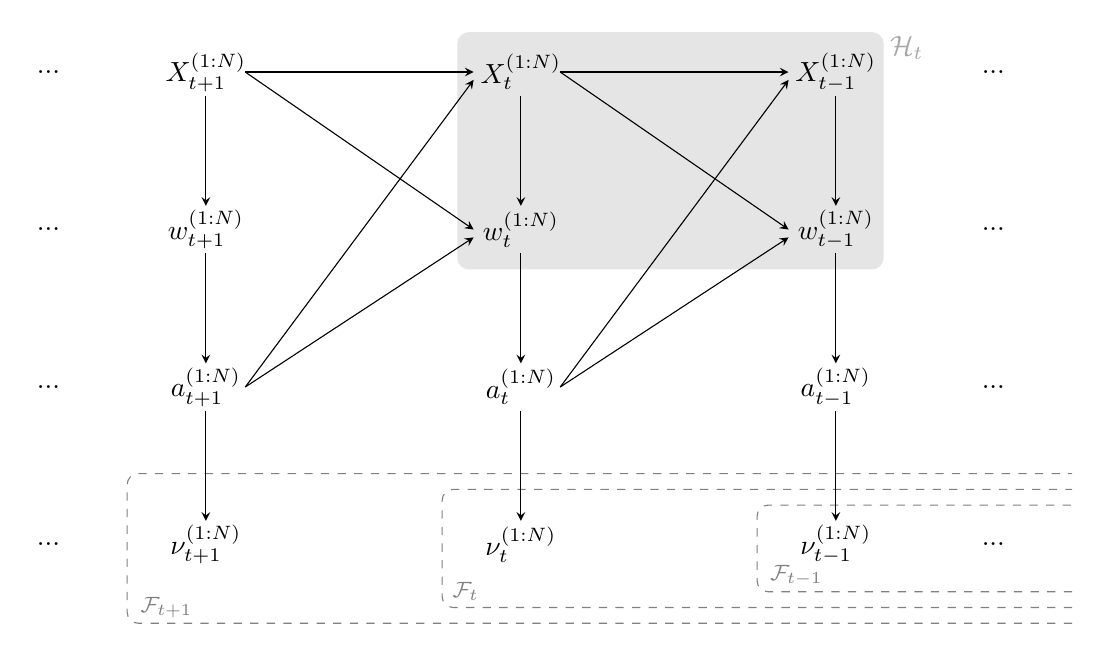
\begin{tikzpicture}[>=stealth]
% separatrix
\filldraw[gray!20, rounded corners] (3.2,0.5)--(8.6,0.5)--(8.6,-2.5)--(3.2,-2.5)--cycle;
\node[gray!70] at (8.9,0.3) {$\mathcal{H}_t$};
% left dots
\node at (-2,0) {...};
\node at (-2,-2) {...};
\node at (-2,-4) {...};
\node at (-2,-6) {...};
% labels (t+1)
\node at (0,0) {$X_{t+1}^{(1:N)}$};
\node at (0,-2) {$w_{t+1}^{(1:N)}$};
\node at (0,-4) {$a_{t+1}^{(1:N)}$};
\node at (0,-6) {$\nu_{t+1}^{(1:N)}$};
% labels t
\node at (4,0) {$X_{t}^{(1:N)}$};
\node at (4,-2) {$w_{t}^{(1:N)}$};
\node at (4,-4) {$a_{t}^{(1:N)}$};
\node at (4,-6) {$\nu_{t}^{(1:N)}$};
% labels (t-1)
\node at (8,0) {$X_{t-1}^{(1:N)}$};
\node at (8,-2) {$w_{t-1}^{(1:N)}$};
\node at (8,-4) {$a_{t-1}^{(1:N)}$};
\node at (8,-6) {$\nu_{t-1}^{(1:N)}$};
% right dots
\node at (10,0) {...};
\node at (10,-2) {...};
\node at (10,-4) {...};
\node at (10,-6) {...};
%filtrations
\draw [rounded corners, dashed, gray] (11,-6.6)--(7,-6.6)--(7,-5.5)--(11,-5.5);
\draw [rounded corners, dashed, gray] (11,-6.8)--(3,-6.8)--(3,-5.3)--(11,-5.3);
\draw [rounded corners, dashed, gray] (11,-7)--(-1,-7)--(-1,-5.1)--(11,-5.1);
% filtration labels
\node[gray] at (7.5,-6.4) {\footnotesize{$\mathcal{F}_{t-1}$}};
\node[gray] at (3.3,-6.6) {\footnotesize{$\mathcal{F}_{t}$}};
\node[gray] at (-0.5,-6.8) {\footnotesize{$\mathcal{F}_{t+1}$}};
% arrows (t+1) -> t
\draw[->] (0.5,0)--(3.4,0);
\draw[->] (0.5,0)--(3.4,-2);
\draw[->] (0.5,-4)--(3.4,-2.1);
\draw[->] (0.5,-4)--(3.4,-0.1);
% arrows t -> (t-1)
\draw[->] (4.5,0)--(7.4,0);
\draw[->] (4.5,0)--(7.4,-2);
\draw[->] (4.5,-4)--(7.4,-2.1);
\draw[->] (4.5,-4)--(7.4,-0.1);
% vertical arrows (t+1)
\draw[->] (0,-0.3)--(0,-1.7);
\draw[->] (0,-2.3)--(0,-3.7);
\draw[->] (0,-4.3)--(0,-5.7);
% vertical arrows t
\draw[->] (4,-0.3)--(4,-1.7);
\draw[->] (4,-2.3)--(4,-3.7);
\draw[->] (4,-4.3)--(4,-5.7);
% vertical arrows (t-1)
\draw[->] (8,-0.3)--(8,-1.7);
\draw[->] (8,-2.3)--(8,-3.7);
\draw[->] (8,-4.3)--(8,-5.7);
\end{tikzpicture}
\caption[Conditional dependence structure of SMC algorithm]{Part of the conditional dependence graph implied by Algorithm \ref{alg:SMC}. The direction of time is from left to right. The reverse-time filtration is indicated by the dashed areas. The nodes highlighted in grey generate the separatrix $\mathcal{H}_t$ between $a_t^{(1:N)}$ and $\mathcal{F}_{t-1}$.\seb{Use the same shades of grey here as elsewhere}}
\label{fig:cond_indep_graph}
\end{figure}


\subsection{Theoretical justification}
\draft{How come SMC works? Convergence results (briefly!) e.g. Lp bounds, CLT, stability.}


\section{Coalescent theory \seb{$\checkmark$} }\label{sec:coaltheory}
\draft{Write a paragraph introducing the section.}

\subsection{Kingman's coalescent}
The Kingman coalescent \parencite{kingman1982gene, kingman1982coal, kingman1982exch} is a continuous-time Markov process on the space of partitions of $\mathbb{N}$. For our purposes we need only consider its restriction to $\{1,\dots,n\}$, termed the $n$-coalescent (defined below), since we only ever consider finite samples from a population. 
However, an excellent probabilistic introduction to the Kingman coalescent from the point-of-view of exchangeable random partitions can be found in \textcite[Chapters 1--2]{berestycki2009}. \seb{or \textcite{wakeley2009} ? or \textcite{durrett2008} ?}
\begin{defn}%[Kingman's $n$-coalescent]
\label{def:kingman}
The \emph{$n$-coalescent} is the homogeneous continuous-time Markov process on the set of partitions of $\{1,\dots,n\}$ with infinitesimal generator $Q$ having entries
\begin{equation}\label{eq:KCgenerator}
q_{\xi,\eta} = \begin{cases}
1 & \xi \prec \eta\\
-|\xi|(|\xi|-1)/2 & \xi=\eta \\
0 & \text{otherwise}
\end{cases}
\end{equation}
where $\xi$ and $\eta$ are partitions of $\{1,...,n\}$, $|\xi|$ denotes the number of blocks in $\xi$, and $\xi \prec \eta$ means that $\eta$ is obtained from $\xi$ by merging exactly one pair of blocks.
\end{defn}

\begin{figure}
\centering
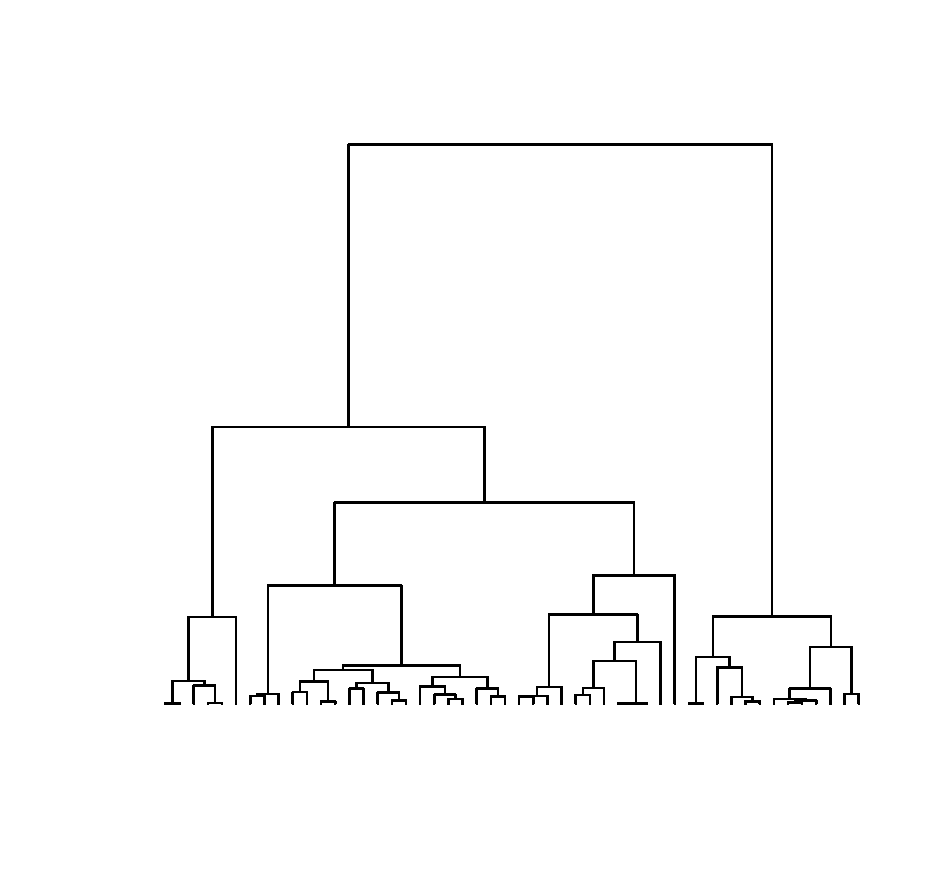
\includegraphics[width=0.6\textwidth, trim={2.8cm 3cm 1.5cm 2cm}, clip]{plots/ncoalescent.pdf}
\caption[The $n$-coalescent]{A realisation of the $n$-coalescent with $n=50$.}
\end{figure}

A particularly attractive feature of the $n$-coalescent is its tractability; its distribution and those of many statistics of interest are available in closed form (Section \ref{sec:KCproperties}).
It turns out also to be extremely useful as a limiting distribution in population genetics, including the genealogies of a wide range of population models in its domain of attraction (Section \ref{sec:popgenmodels}).


\subsection{Properties of Kingman's coalescent}\label{sec:KCproperties}
The simplicity of $Q$ allows various properties of the $n$-coalescent to be studied analytically. \seb{Refer to more exhaustive studies of the properties in the literature, e.g.\ \textcite[Section 1.2]{durrett2008}.}
Starting with $n$ blocks, exactly $n-1$ coalescences are required to reach the absorbing state where all blocks have coalesced, known in the population genetics literature as the \emph{most recent common ancestor} (MRCA).

\begin{figure}[ht]
\centering
\begin{tikzpicture}
% horizontal lines
\draw[dotted, gray] (-0.5,-1)--(6,-1);
\draw[dotted, gray] (-0.5,-0.2)--(6,-0.2);
\draw[dotted, gray] (-0.5,0.5)--(6,0.5);
\draw[dotted, gray] (-0.5,1.3)--(6,1.3);
\draw[dotted, gray] (-0.5,3.3)--(6,3.3);

% tree
\draw[thick] (0,-1)--(0,-0.2);
\draw[thick] (1,-1)--(1,-0.2);
\draw[thick] (0,-0.2)--(1,-0.2);
\draw[thick] (0.5,-0.2)--(0.5,1.3);
\draw[thick] (2,-1)--(2,1.3);
\draw[thick] (0.5,1.3)--(2,1.3);
\draw[thick] (3,-1)--(3,0.5);
\draw[thick] (4,-1)--(4,0.5);
\draw[thick] (3,0.5)--(4,0.5);
\draw[thick] (1.25,1.3)--(1.25,3.3);
\draw[thick] (3.5,0.5)--(3.5,3.3);
\draw[thick] (1.25,3.3)--(3.5,3.3);

% interval arrows
\draw[<->] (5,-1)--(5,-0.2);
\draw[<->] (5,-0.2)--(5,0.5);
\draw[<->] (5,0.5)--(5,1.3);
\draw[<->] (5,1.3)--(5,3.3);

% small t's
\node at (5.2, -0.6) {\footnotesize{$t_5$}};
\node at (5.2, 0.15) {\footnotesize{$t_4$}};
\node at (5.2, 0.9) {\footnotesize{$t_3$}};
\node at (5.2, 2.3) {\footnotesize{$t_2$}};

% capital T's
\node[anchor=west] at (6, -1) {\footnotesize{$T_5 = 0$}};
\node[anchor=west] at (6, -0.2) {\footnotesize{$T_4$}};
\node[anchor=west] at (6, 0.5) {\footnotesize{$T_3$}};
\node[anchor=west] at (6, 1.3) {\footnotesize{$T_2$}};
\node[anchor=west] at (6, 3.3) {\footnotesize{$T_1 = T_{MRCA}$}};
\end{tikzpicture}
\caption{Diagram illustrating the definitions of $t_i$, $T_i$ in the $n$-coalescent.}
\label{fig:KC_timedefns}
\end{figure}

Denote by $t_2, t_3 \dots, t_n$ the waiting times between coalescent events, where $t_i$ is the amount of time for which the coalescent has exactly $i$ distinct lineages (see Figure~\ref{fig:KC_timedefns}).
A consequence of Definition~\ref{def:kingman} is that these waiting times are independent and have distributions
\begin{equation}
t_i \sim \Exp\left( \binom{i}{2} \right) .
\end{equation}
The partial sum $T_k := \sum_{i=k+1}^n t_i$ gives the total time up to the $(n-k)^{th}$ coalescence event, i.e.\ the first time at which there are only $k$ lineages remaining out of the initial $n$ (see Figure~\ref{fig:KC_timedefns}).
The partial sums, being sums of independent Exponential random variables, have HyperExponential distributions.

\seb{Refer back to the following three properties later on with reference to their relevance in SMC.}

\subsubsection{Time to MRCA}
Of particular interest is the tree height or time to the most recent common ancestor, $T_{MRCA} := T_1$.
With some algebra we find, for instance,
\begin{equation}
\E[ T_{MRCA} ] 
= \sum_{i=2}^{n} \E[t_i]
= \sum_{i=2}^n \frac{2}{i(i-1)}
= 2 \sum_{i=2}^n \left\{ \frac{1}{i-1} - \frac{1}{i} \right\}
= 2 \left( 1 - \frac{1}{n} \right)
\end{equation}
and
\begin{equation}
\V[ T_{MRCA} ] 
= \sum_{i=2}^n \V[t_i]
= \sum_{i=2}^n \left( \frac{2}{i(i-1)} \right)^2 .
\end{equation}
The expected tree height converges to 2 as $n\to\infty$, and the variance converges to $4(\pi^2 - 9)/3 \simeq 1.16$.
The somewhat surprising fact that the tree height does not diverge with $n$ is a result of the very high rate of coalescence close to the bottom of the tree. This rate is large enough that the full Kingman coalescent (on $\mathbb{N}$) \emph{comes down from infinity}, that is, despite starting with infinitely many blocks, after any positive amount of time these have coalesced into finitely many blocks.
\seb{Plot mean with sd-ribbon over $n$ for an illustration? SD ribbon isn't the right thing; since we apparently know the actual distribution, plot a high density interval of that. (also for $L$)}


\subsubsection{Total branch length}
Another quantity of interest is the total branch length,
$ L := \sum_{i=2}^n i t_i $.
For instance
\begin{equation}
\E[ L ] 
= \sum_{i=2}^n i \E[ t_i ]
= \sum_{i=2}^n \frac{2}{i-1}
= \sum_{i=1}^{n-1} \frac{2}{i} %,
\simeq 2 \ln(n-1) 
\end{equation}
%a harmonic series, 
and
\begin{equation}
\V[ L ] 
= \sum_{i=2}^n i^2 \V[ t_i ]
= \sum_{i=2}^n \frac{4}{(i-1)^2}
= \sum_{i=1}^{n-1} \frac{4}{i^2} .
\end{equation}
Note that although the mean total branch length diverges with $n$, the variance converges to a constant, $4\pi /6 \simeq 6.6$.


\subsubsection{Probability that sample MRCA equals population MRCA}
One other interesting quantity is the probability that the MRCA of $k$ random lineages coincides with the population MRCA \parencite[e.g.][Theorem 1.7]{durrett2008}.
Denote by $S_k$ the relevant event: that a random sample of $k$ lineages has the same as the MRCA as the population.
Consider the two subtrees produced by cutting the tree just below the population MRCA. The sample of $k$ lineages coalesces before the population MRCA if and only if all $k$ sampled leaves lie in just one of these two subtrees.
A basic consequence of the exchangeability of the $n$-coalescent is that, in the limit $N\to\infty$, the proportion of leaves in the left subtree is uniformly distributed on $[0,1]$.
Calling this proportion $X$, we have
\begin{equation*}
\Prob [ S_k^c \mid X=x]
= x^k + (1-x)^k
\end{equation*}
Integrating against the distribution of $X$, the probability of interest is
\begin{equation*}
\Prob[ S_k ]
= 1- \int_0^1 [ x^k + (1-x)^k ] dx
= \frac{k-1}{k+1}
\end{equation*}
as required.

The above is based on properties of the full Kingman coalescent, but similar results are available for the $n$-coalescent.
Consider now a subsample of size $k$ among $n$ lineages that follow the $n$-coalescent.
Denote by $S_{k,n}$ the event that these $k$ lineages have the same MRCA as all $n$ lineages.
This probability of this event is calculated in \textcite[Example 1]{saunders1984} and again in \textcite[Equation (3)]{spouge2014}, in both cases arising as a special case of more general results. A direct proof is given below.

Let $X$ be the number of leaves in the left subtree. So $X \in \{1,\dots,n-1\} $ and, like before, a consequence of exchangeability is that $X$ is uniformly distributed on that set.
Now that the total number of branches is finite, we have to count more carefully. Conditional on $X$ we have
\begin{equation*}
\Prob [S_{k,n}^c \mid X=x]
= \left[ \binom{x}{k} + \binom{n-x}{k} \right] \binom{n}{k}^{-1} .
\end{equation*}
Integrating against the distribution of $X$ gives
\begin{align*}
\Prob[ S_{k,n} ]
&= 1 - \frac{1}{n-1} \binom{n}{k}^{-1} \, \sum_{x=1}^{n-1} 
        \left[ \binom{x}{k} + \binom{n-x}{k} \right] \\
&= 1 - \frac{1}{n-1} \binom{n}{k}^{-1} 
        \left[ \binom{n}{k+1} + \binom{n}{k+1} \right] \\
&= \frac{k-1}{k+1} \frac{n+1}{n-1}
\end{align*}
using binomial identities and some algebra.
As $n\to\infty$ this agrees with the population-level result above.



\subsection{Models in population genetics}\label{sec:popgenmodels}
The Kingman coalescent is the limiting coalescent process (in the large population limit) for a surprisingly wide range of population models. Some important examples of models in Kingman's ``domain of attraction'' are introduced in this section.
Common to all of these models are the following assumptions:
\begin{itemize}
\item The population has constant size $N$
\item Reproduction happens in discrete generations
\item The offspring distributions are identical at each generation, and independent between generations
\item These models are all \emph{neutral}, i.e.\ the offspring distribution is exchangeable.
\end{itemize}
As before \seb{section/eq ref?}, we define offspring counts in terms of parental indices as $\nu_j := |\{ i: a_i = j\}|$.
Under the assumption of neutrality, it is sufficient to consider only the offspring counts, rather than the parental indices (which generally carry more information).
\seb{Crucially, in the neutral case, offspring counts carry all the information about the distribution of the genealogy that is contained in the parental indices.}
From a biological perspective, neutrality encodes the absence of natural selection, i.e.\ no individual in the population is ``fitter'' than another.

\subsubsection{Wright-Fisher model}
The neutral Wright-Fisher model \parencite{fisher1923, fisher1930, wright1931} is one of the most studied models in population genetics.
At each time step the existing generation dies and is replaced by $N$ offspring. The offspring descend from parents $(a_1, \dots, a_N)$ which are selected according to
\begin{equation*}
a_i \overset{iid}{\sim} \Cat(\{1, \dots, N\}, (1/N, \dots, 1/N)).
\end{equation*}
The joint distribution of the offspring counts is therefore
\begin{equation*}
(v_1,\dots, v_N) \sim \Mn(N, (1/N, \dots, 1/N)).
\end{equation*}
Since the Multinomial distribution is exchangeable, this model is neutral.
There are several non-neutral variants of the Wright-Fisher model \seb{citations?}, but they are typically much less tractable than the neutral one.

Kingman showed in his original papers introducing the Kingman coalescent \parencite{kingman1982gene} that, when time is scaled by a factor of $N$, genealogies of the neutral Wright-Fisher model converge to the Kingman coalescent as $N\to\infty$.

\subsubsection{Cannings model}
The neutral Cannings model \parencite{cannings1974, cannings1975} is a more general construction which encompasses the neutral Wright-Fisher model as a special case.

In the Cannings model, the particular offspring distribution is not specified; we only require that it is exchangeable, i.i.d.\ between generations, and preserves the population size. In particular, the probability of observing offspring counts $(v_1, \dots, v_N)$ must be invariant under permutations of this vector.

Genealogies of the neutral Cannings model also converge to the Kingman coalescent, under some conditions and a suitable time-scaling \seb{which is what?}, as $N\to\infty$ \parencite[see for example][Section 2.2]{etheridge2011}. \seb{original reference for this? is not any Kingman 1982 papers, and certainly not Cannings 1974/5 which predates KC}

\subsubsection{Moran model}
The neutral Moran model \parencite{moran1958}, while perhaps less biologically relevant, is mathematically appealing because its simple dynamics make it particularly tractable.

At each time step, an ordered pair of individuals is selected uniformly at random. The first individual in this pair dies (i.e.\ leaves no offspring in the next generation), while the other reproduces (leaving two offspring). All of the other individuals leave exactly one offspring.
%Usually the model is thought of as having ``overlapping generations'': the individuals having one offspring are considered to be not reproducing but rather surviving to appear again in the next generation.
%However, one can equally think of it as having non-overlapping generations and a low variance reproduction mechanism.
This is another special case of the neutral Cannings model, where the offspring distribution is now uniform over all permutations of $(0,2,1,1,\dots,1)$.
Therefore we know that under a suitable time-scaling, its genealogies converge to the Kingman coalescent. The time scale in this case is $N^2$, because reproduction happens at a rate $N$ times \seb{or is it technically N-1 times?} lower than in the Wright-Fisher model. \seb{also cite a Moran-specific convergence result: not sure where (it isn't in Kingman 1982* or in Moran 1958 which predates KC)}


\subsection{Particle populations}
Much of the population genetics framework transfers readily to the case of SMC. The population is now a population of particles, with each iteration of the SMC algorithm corresponding to a generation, and resampling playing the part of reproduction.
In fact, SMC ``populations'' are in some ways more suited to these population models than actual populations of organisms.
The assumptions that the population has constant size $N$ and that reproduction occurs only at discrete generations are satisfied by construction.
However, we cannot assume independence between generations: as seen in Figure~\ref{fig:cond_indep_graph}, the offspring counts at subsequent generations are not independent without some conditioning. In fact, after marginalising out the information about the positions of the particles, the genealogical process is not even Markovian.
Nor is our model neutral: the resampling distribution depends on the weight of each particle (the weight plays the role of fitness in a non-neutral population model).






\section{Sequential Monte Carlo genealogies}

\subsection{From particles to genealogies}
\draft{How does the SMC algorithm induce a genealogy? (resampling = parent-child relationship).}

\subsection{Performance}
\draft{How do genealogies affect performance? Variance (and variance estimation?), storage cost. Ancestral degeneracy.}

\begin{figure}[ht]
\centering
\subfloat[Multinomial resampling]{
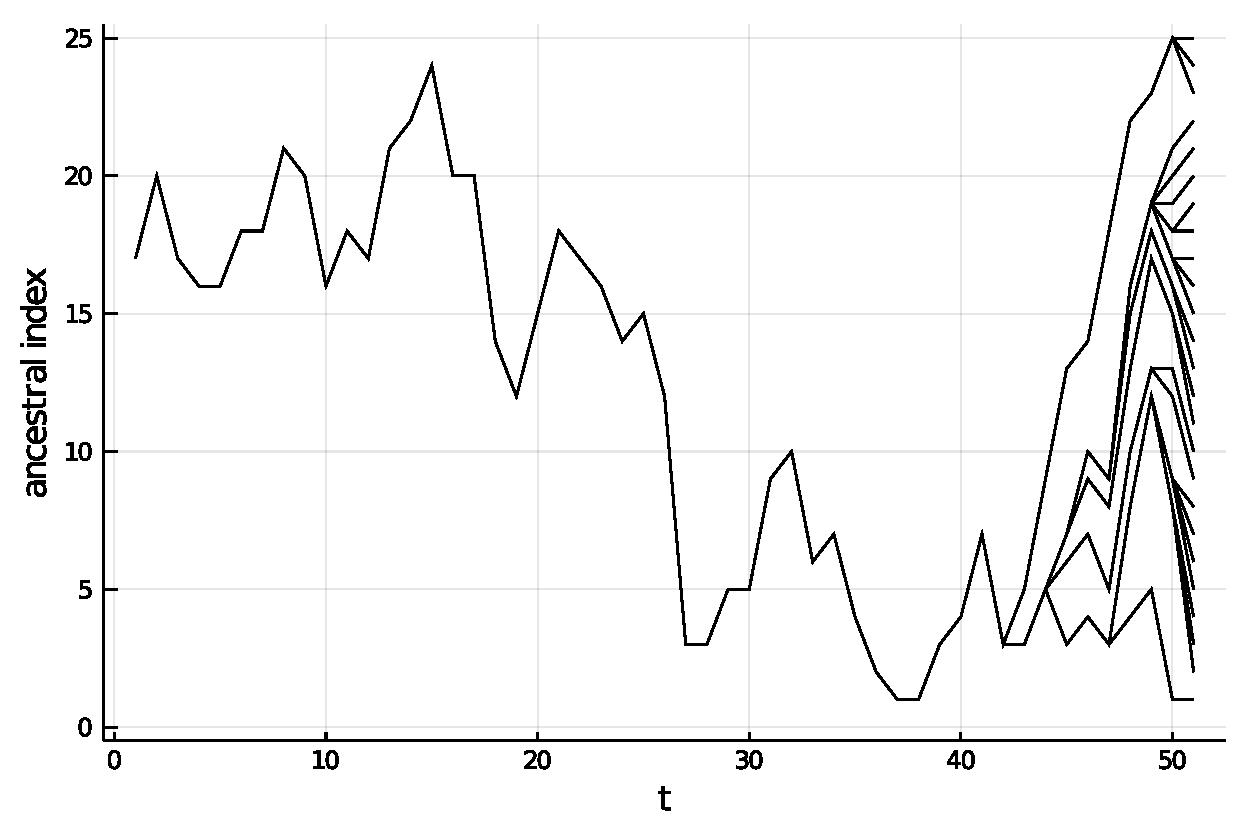
\includegraphics[width=0.5\textwidth]{plots/ancdegen_mn.pdf}
\label{fig:ancdegen_mn}
}
\subfloat[Adaptive minimum-variance resampling]{
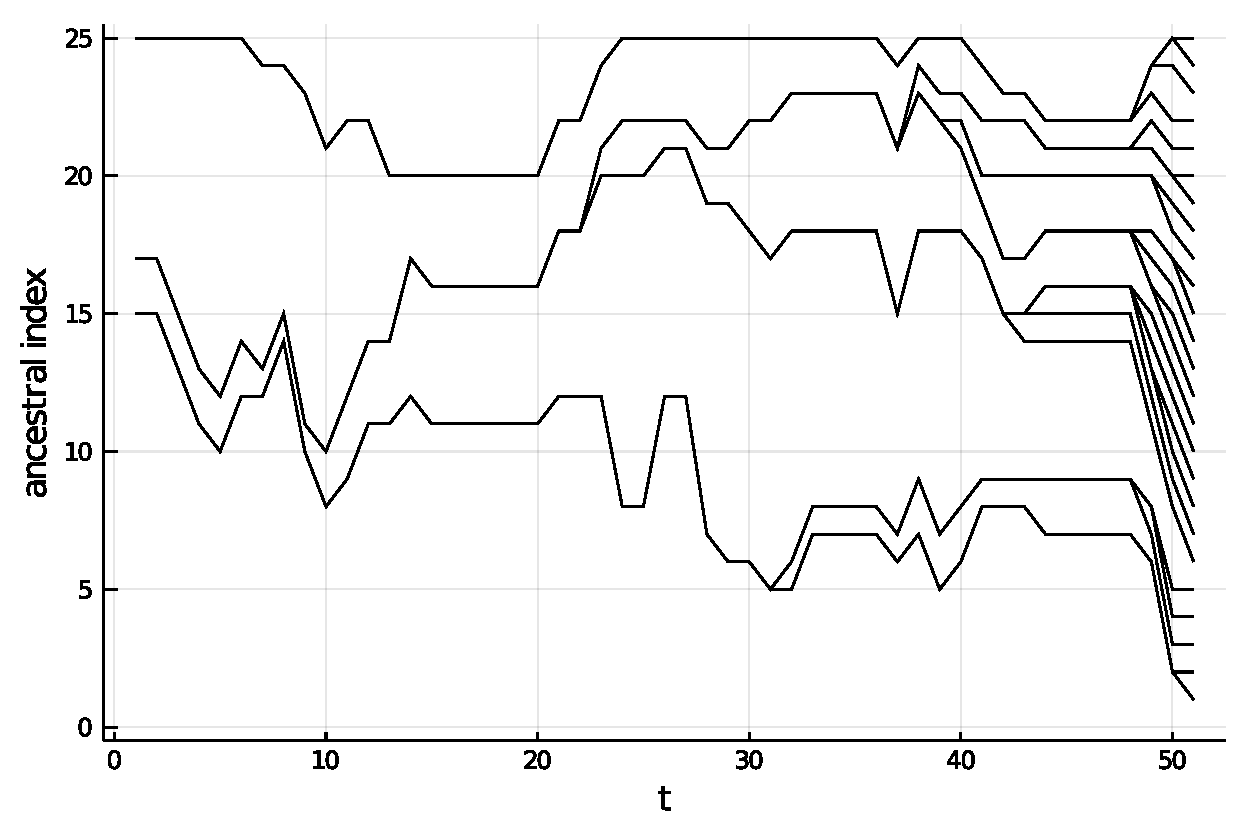
\includegraphics[width=0.5\textwidth]{plots/ancdegen_adaptsyst.pdf}
\label{fig:ancdegen_adaptsyst}
}
\caption[Ancestral degeneracy illustration]{Illustration of ancestral degeneracy and the mitigating effect of low-variance and adpative resampling. \subref{fig:ancdegen_mn} with multinomial resampling, \subref{fig:ancdegen_adaptsyst} the same system with adaptive systematic resampling.}
\label{fig:ancestral_degeneracy}
\end{figure}

\subsection{Mitigating ancestral degeneracy}
\draft{Low-variance resampling (save details for next section). Adaptive resampling: idea of balancing weight/ancestral degeneracy; rule of thumb for implementing it; when is it effective or not?; necessary changes to our generic SMC algorithm (calculation of weights in particular). Backward sampling: when is it possible to do this?}

\subsection{Asymptotics}
\draft{Why are large population asymptotics useful? Existing results (path storage, KJJS).}



\section{Resampling \seb{$\sim$} }
As we have seen, resampling is necessary within SMC to ``reset'' the weights in order to prevent weight degeneracy.
The basic role of a resampling scheme is to map the continuous weights to discrete offspring counts, in some ``sensible'' way (Definition~\ref{defn:resampling}).
The choice of resampling scheme is explored in detail in this section.
%There are other considerations when choosing between the many possible resampling schemes; some of these are explored in Section~\ref{sec:resampling_properties}, and some popular choices of resampling scheme are described in Section~\ref{sec:examples_resamplingschemes}.

\subsection{Definition \seb{$\checkmark$} }
\draft{Also say that resampling is itself a Monte Carlo procedure.}

\begin{defn}\label{defn:resampling}
For our purposes, a valid resampling scheme is a stochastic function mapping weights 
$w_t^{(1:N)} \in \mathcal{S}_{N-1}$ 
to offspring counts 
$\nu_t^{(1:N)} \in \{0,\dots,N\}^N $
that satisfies the following properties:
\begin{enumerate}
\item\label{item:resampling_property1} the population size is conserved:
$ \sum_{i=1}^N \nu_t^{(i)} =N $ for all $N$
\item\label{item:resampling_property2} the weights are uniform after resampling:
$w_{t+}^{(i)} = 1/N$ for all $i$
\item\label{item:resampling_property3} the resampling is unbiased:
$ \E[ \nu_t^{(i)} \mid w_t^{(i)} ] = N w_t^{(i)} $ for all $i$.
\end{enumerate}
\end{defn}
It is possible to design resampling schemes that violate these properties.
For example, a scheme of \textcite{liu1998} uses the square roots of the weights for resampling, then corrects by setting non-uniform weights after resampling (violating conditions \ref{item:resampling_property2} and \ref{item:resampling_property3}).
\seb{\textcite[p.890, point (d)]{fearnhead2003} also appears to resample such that the weights are not uniform after resampling.}
%
Resampling different numbers of particles in different iterations (violating condition \ref{item:resampling_property1}) is of course possible, but we typically have a fixed limit on computational resources, in which case it makes sense to simulate the maximum feasible number of particles $N$ at every iteration.
%
Deterministic resampling schemes (which cannot generally be unbiased, violating condition \ref{item:resampling_property3}) have been used by some authors. These include schemes based on optimal transport \parencite{reich2013, myers2021, corenflos2021} and the importance support points resampling of \textcite{huang2020}.
However, the majority of resampling schemes in the literature fit within Definition~\ref{defn:resampling}, and it is not typically advantageous to violate the properties \ref{item:resampling_property1}--\ref{item:resampling_property3}.

Within Definition~\ref{defn:resampling} there is still a great deal of flexibility. Many different resampling schemes have been proposed in the literature, some of which perform better than others.
 Section~\ref{sec:examples_resamplingschemes} introduces some important resampling schemes, and their properties are discussed in Section~\ref{sec:resampling_properties}. 
These are summarised in Table~\ref{tab:resampling_properties}.



\subsection{Examples \seb{$\sim$} }\label{sec:examples_resamplingschemes}
\draft{Argue in each case that the scheme is unbiased.}

\begin{table}[ht]
\centering
\begin{tabular}{ l l }
\hline\hline
Abbreviation & Description \\% & Defined in Section \\
\hline
\texttt{multi} & multinomial resampling \\%& \ref{sec:resampling_multinomial} \\
\texttt{star} & star resampling \\%& \ref{sec:resampling_star} \\
\texttt{strat} & stratified resampling \\%& \ref{sec:resampling_stratified} \\
\texttt{syst} & systematic resampling \\%& \ref{sec:resampling_systematic} \\
\texttt{res-multi} & residual resampling with multinomial residuals \\
        %& \ref{sec:resampling_residual} \\
\texttt{res-star} & residual resampling with star residuals \\
        %& \ref{sec:resampling_residual} \\
\texttt{res-strat} & residual resampling with stratified residuals \\
        %& \ref{sec:resampling_residual} \\
\texttt{res-syst} & residual resampling with systematic residuals \\
        %& \ref{sec:resampling_residual} \\
\texttt{ssp} & Srinivasan sampling procedure resampling \\%& \\
\texttt{branch} & minimal variance branching algorithm \\%& \\
\hline\hline
\end{tabular}
\caption{Abbreviations for resampling schemes}
\label{tab:resampling_abbrevs}
\end{table} 


 
\subsubsection{Multinomial resampling \seb{$\checkmark$} }%\label{sec:resampling_multinomial}
Multinomial resampling \parencite{gordon1993,efron1994} is one of the simplest resampling schemes.
The parental indices are chosen independently from $\{1, \dots, N\}$, each with probability given by the weight of the corresponding particle $w_t^{(i)}$. 
That is, 
\begin{equation*}
a_t^{(1:N)} \sim \Cat( \{1,\dots, N\}, w_t^{(1:N)} ) .
\end{equation*}
This implies the joint distribution of the offspring counts is 
\begin{equation*}
\nu_t^{(1:N)} \eqdist \operatorname{Multinomial}(N, w_t^{(1:N)} ) .
\end{equation*}
It follows from the mean of the Multinomial distribution that this resampling scheme is unbiased.
\seb{Although the parental indices are chosen independently, the resulting offspring counts are negatively correlated. --- link to GCW19's negative association?}

A simple way to sample the parental indices is to use inversion sampling: partition the unit interval into $N$ subintervals each of which will correspond to a certain index $i$ and has length equal to the weight $w_t^{(i)}$; then draw $N$ samples $U_i \sim \Unif(0,1)$ and classify them according to which of these subintervals they fall in.
Explicitly, the parental index assigned to child $i$ is the index $a_i$ satisfying
\begin{equation}\label{eq:syst_strat_resampling}
\sum_{j=1}^{a_i -1} w_t^{(j)} \leq U_i \leq \sum_{j=1}^{a_i} w_t^{(j)} .
\end{equation}
This is illustrated in Figure \ref{fig:resampling_mn}. 
%Note that there exist more efficient methods to sample from a Multinomial distribution, so the inversion method may not be used in practice.

Fast implementations of multinomial resampling rely on $U_1,\dots,U_N$ being pre-sorted, which speeds up the search step \eqref{eq:syst_strat_resampling}. Sorting $N$ numbers is an $O(N\log N)$ operation, but in fact this is not necessary because we can directly sample the order statistics of a $\Unif[0,1]$ distribution \seb{[citations: \textcite{chopin2020}, and a different (or possibly equivalent) method in \textcite{hol2006}] ---explore whether these methods are equivalent}.
This allows multinomial resampling to be implemented at $O(N)$ cost, with the side-effect that the sampled ancestral indices will be ordered. \seb{And therefore the sampled parental indices cannot be Cat(N,w) distributed. But the counts are still Multinomial? And anyway for the purposes of resampling this isn't a problem; it might even improve performance?}


\subsubsection{Residual resampling \seb{$\checkmark$} }%\label{sec:resampling_residual}
Residual resampling is described in \textcite{liu1998} and also in \textcite{whitley1994} where it is called ``remainder stochastic sampling''.

Each particle $X_{t}^{(i)}$ is deterministically assigned $\flnw$ offspring and the remaining $R := \sum_{i=1}^N ( Nw_t^{(i)} - \flnw) = n                           N- \sum_{i=1}^N \flnw$ offspring are assigned stochastically according to the residual weights
\begin{equation*}
r^{(i)} := ( Nw_t^{(i)} - \flnw) /R .
\end{equation*}
Notice that each $r^{(i)}$ lies in the interval $(0, 1/R)$.

The stochastic part can be done using any of the other basic resampling schemes (e.g.\ multinomial, stratified, systematic). Most presentations focus on the case where multinomial resampling is used for the residuals, which is by no means the most sensible option. We will explore several different options in what follows.

%This yields a vector of offspring counts
%\begin{equation*}
%\nu_t^{(1:N)} \eqdist \lfloor N w_t^{(1:N)} \rfloor +  \operatorname{Multinomial}(R, (N w_t^{(1:N)} - \lfloor N w_t^{(1:N)}\rfloor)/R) .
%\end{equation*}
%The deterministic part ensures that every particle with weight $>1/N$ is guaranteed to survive. This is a desirable property as it prevents the random loss of high-weighted particles.



\begin{figure}
\centering
\subfloat[Multinomial resampling]{
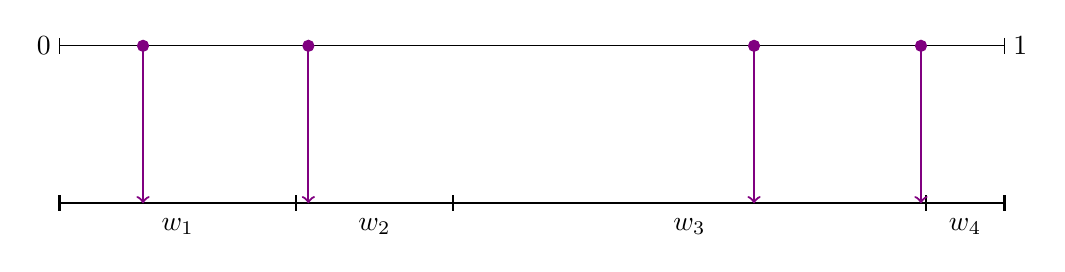
\begin{tikzpicture}
%parallel lines
\draw[thick] (0,0) -- (12,0);
\draw (0,2) -- (12,2);
% tick marks at ends
\draw[thick] (0,0.1) --(0,-0.1);
\draw[thick] (12,0.1) --(12,-0.1);
\draw (0,2.1) --(0,1.9);
\draw (12,2.1) --(12,1.9);
% tick marks indicating weights
\draw[thick] (3,0.1) --(3,-0.1);
\draw[thick] (5,0.1) --(5,-0.1);
\draw[thick] (11,0.1) --(11,-0.1);
% weight labels
\node at (1.5,-0.3) {$w_1$};
\node at (4,-0.3) {$w_2$};
\node at (8,-0.3) {$w_3$};
\node at (11.5,-0.3) {$w_4$};
% endpoint labels
\node at (-0.2,2) {$0$};
\node at (12.2,2) {$1$};
% uniform points
\filldraw[violet] (10.94,2) circle (2pt);
\filldraw[violet] (1.06,2) circle (2pt);
\filldraw[violet] (8.82,2) circle (2pt);
\filldraw[violet] (3.16,2) circle (2pt);
% arrows from random points
\draw[thick, violet, ->] (10.94,2) -- (10.94,0);
\draw[thick, violet, ->] (1.06,2) -- (1.06,0);
\draw[thick, violet, ->] (8.82,2) -- (8.82,0);
\draw[thick, violet, ->] (3.16,2) -- (3.16,0);
\end{tikzpicture}
\label{fig:resampling_mn}
}\\
\subfloat[Stratified resampling]{
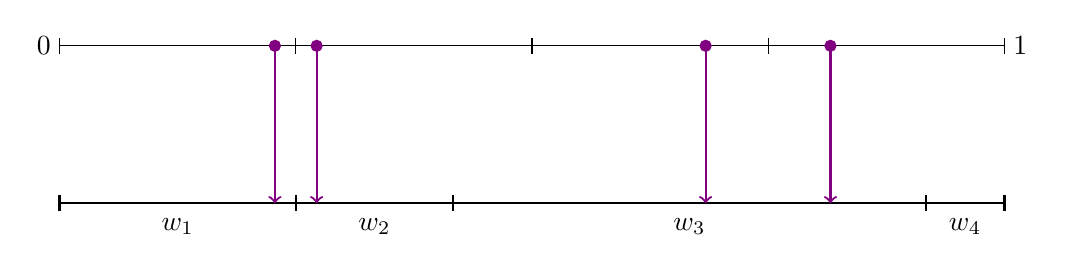
\begin{tikzpicture}
%parallel lines
\draw[thick] (0,0) -- (12,0);
\draw (0,2) -- (12,2);
% tick marks at ends
\draw[thick] (0,0.1) --(0,-0.1);
\draw[thick] (12,0.1) --(12,-0.1);
\draw (0,2.1) --(0,1.9);
\draw (12,2.1) --(12,1.9);
% tick marks indicating weights
\draw[thick] (3,0.1) --(3,-0.1);
\draw[thick] (5,0.1) --(5,-0.1);
\draw[thick] (11,0.1) --(11,-0.1);
% tick marks indicating sampling intervals:
\draw (3,2.1) --(3,1.9);
\draw (6,2.1) --(6,1.9);
\draw (9,2.1) --(9,1.9);
% weight labels
\node at (1.5,-0.3) {$w_1$};
\node at (4,-0.3) {$w_2$};
\node at (8,-0.3) {$w_3$};
\node at (11.5,-0.3) {$w_4$};
% endpoint labels
\node at (-0.2,2) {$0$};
\node at (12.2,2) {$1$};
% stratified points
\filldraw[violet] (2.735,2) circle (2pt);
\filldraw[violet] (3.265,2) circle (2pt);
\filldraw[violet] (8.205,2) circle (2pt);
\filldraw[violet] (9.79,2) circle (2pt);
% arrows from random points
\draw[thick, violet, ->] (2.735,2) -- (2.735,0);
\draw[thick, violet, ->] (3.265,2) -- (3.265,0);
\draw[thick, violet, ->] (8.205,2) -- (8.205,0);
\draw[thick, violet, ->] (9.79,2) -- (9.79,0);
\end{tikzpicture}
\label{fig:resampling_stratified}
}\\
\subfloat[Systematic resampling]{
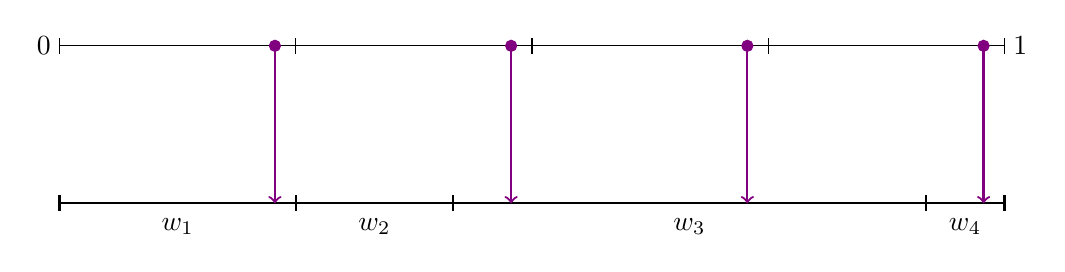
\begin{tikzpicture}
%parallel lines
\draw[thick] (0,0) -- (12,0);
\draw (0,2) -- (12,2);
% tick marks at ends
\draw[thick] (0,0.1) --(0,-0.1);
\draw[thick] (12,0.1) --(12,-0.1);
\draw (0,2.1) --(0,1.9);
\draw (12,2.1) --(12,1.9);
% tick marks indicating weights
\draw[thick] (3,0.1) --(3,-0.1);
\draw[thick] (5,0.1) --(5,-0.1);
\draw[thick] (11,0.1) --(11,-0.1);
% tick marks indicating sampling intervals:
\draw (3,2.1) --(3,1.9);
\draw (6,2.1) --(6,1.9);
\draw (9,2.1) --(9,1.9);
% weight labels
\node at (1.5,-0.3) {$w_1$};
\node at (4,-0.3) {$w_2$};
\node at (8,-0.3) {$w_3$};
\node at (11.5,-0.3) {$w_4$};
% endpoint labels
\node at (-0.2,2) {$0$};
\node at (12.2,2) {$1$};
% stratified points
\filldraw[violet] (2.735,2) circle (2pt);
\filldraw[violet] (5.735,2) circle (2pt);
\filldraw[violet] (8.735,2) circle (2pt);
\filldraw[violet] (11.735,2) circle (2pt);
% arrows from random points
\draw[thick, violet, ->] (2.735,2) -- (2.735,0);
\draw[thick, violet, ->] (5.735,2) -- (5.735,0);
\draw[thick, violet, ->] (8.735,2) -- (8.735,0);
\draw[thick, violet, ->] (11.735,2) -- (11.735,0);
\end{tikzpicture}
\label{fig:resampling_systematic}
}\\
\caption[Resampling using multinomial, stratified and systematic schemes]{Inversion sampling to obtain Multinomial offspring counts, where the (marginally) Uniform variables for inversion are sampled in different ways. For this example $N=4$ and the weights are $w_{(1:4)} = \frac{1}{N}(1,\frac{2}{3},2,\frac{1}{3})$. 
\seb{Also make the same diagram in Whitley's ``roulette wheel'' style, to illustrate the difference. Or maybe make it for the ``degeneracy under equal weights'' section just illustrating the difference it makes in stratified resampling.}
%In each case the samples to be inverted are seeded with the same $\Unif(0,1)$ samples.
%\subref{fig:resampling_mn} Sample $N$  independent $\Unif(0,1)$ random variables. In this example the sampled offspring counts are $(1,1,2,0)$.
%\subref{fig:resampling_stratified} The $\Unif(0,1)$ samples are transformed to Uniform draws from the intervals (0,0.25), (0.25,0.5), (0.5, 0.75), (0.75,1). In this example the sampled offspring counts are $(1,1,2,0)$.
%\subref{fig:resampling_systematic} Use only the first draw and transform it to a sample from $\Unif(0,0.25)$. For the subsequent samples, add 0.25 each time to obtain a sample in each interval. In this example the sampled offspring counts are $(1,0,2,1)$.
}
\end{figure}



\subsubsection{Stratified resampling \seb{$\checkmark$} }%\label{sec:resampling_stratified}
Stratified resampling is introduced in \cite{kitagawa1996}.

As in multinomial resampling, stratified resampling uses inversion sampling to dample the parental indices. However, the samples used for inversion sampling are no longer i.i.d. $\Unif[0,1]$ samples. Instead, one number is sampled from each subinterval of length $1/N$; that is, 
\begin{equation*}
U_i \sim \Unif \left(\frac{i-1}{N}, \frac{i}{N} \right) .
\end{equation*}
Alternatively, one may think of standard Uniform samples $u_1,\dots,u_N \sim^{iid} \Unif[0,1]$ with the transformation
\begin{equation*}
U_i = \frac{u_i + i -1}{N}
\end{equation*}
to give the stratified samples $U_1,\dots,U_N$.

The parents are then assigned as in \eqref{eq:syst_strat_resampling}.
This is illustrated in Figure \ref{fig:resampling_stratified}.
The offspring distribution is no longer Multinomial, since parental indices are not chosen independently.
This scheme ensures that the samples are ``well spread out'', which reduces the probability of randomly losing high-weight particles or duplicating low-weight particles.

It will be useful later on to have a better idea about the marginal distributions of $\nu_t^{(i)}$ that are induced by stratified resampling. There are complex dependencies between the offspring counts, but we can still find some constraints on the distribution of each count conditional on the corresponding weight.
Write the $i^{th}$ weight in the form $w_t^{(i)} = (k + \delta)/N$, where $\delta \in [0,1)$ and $k\in \{0,\dots,N-1\}$.
Considering the illustration Figure~\ref{fig:resampling_stratified}, the distribution of $\nu_t^{(i)}$ depends not only on $w_t^{(i)}$ but also on where the $i^{th}$ weight interval falls with respect to the length-$(1/N)$ intervals. There are two cases to consider, which are illustrated in Figure~\ref{fig:strat_cases}. Note that Case \subref{fig:strat_case2} cannot happen if $k=0$.

%\begin{figure}
%\centering
%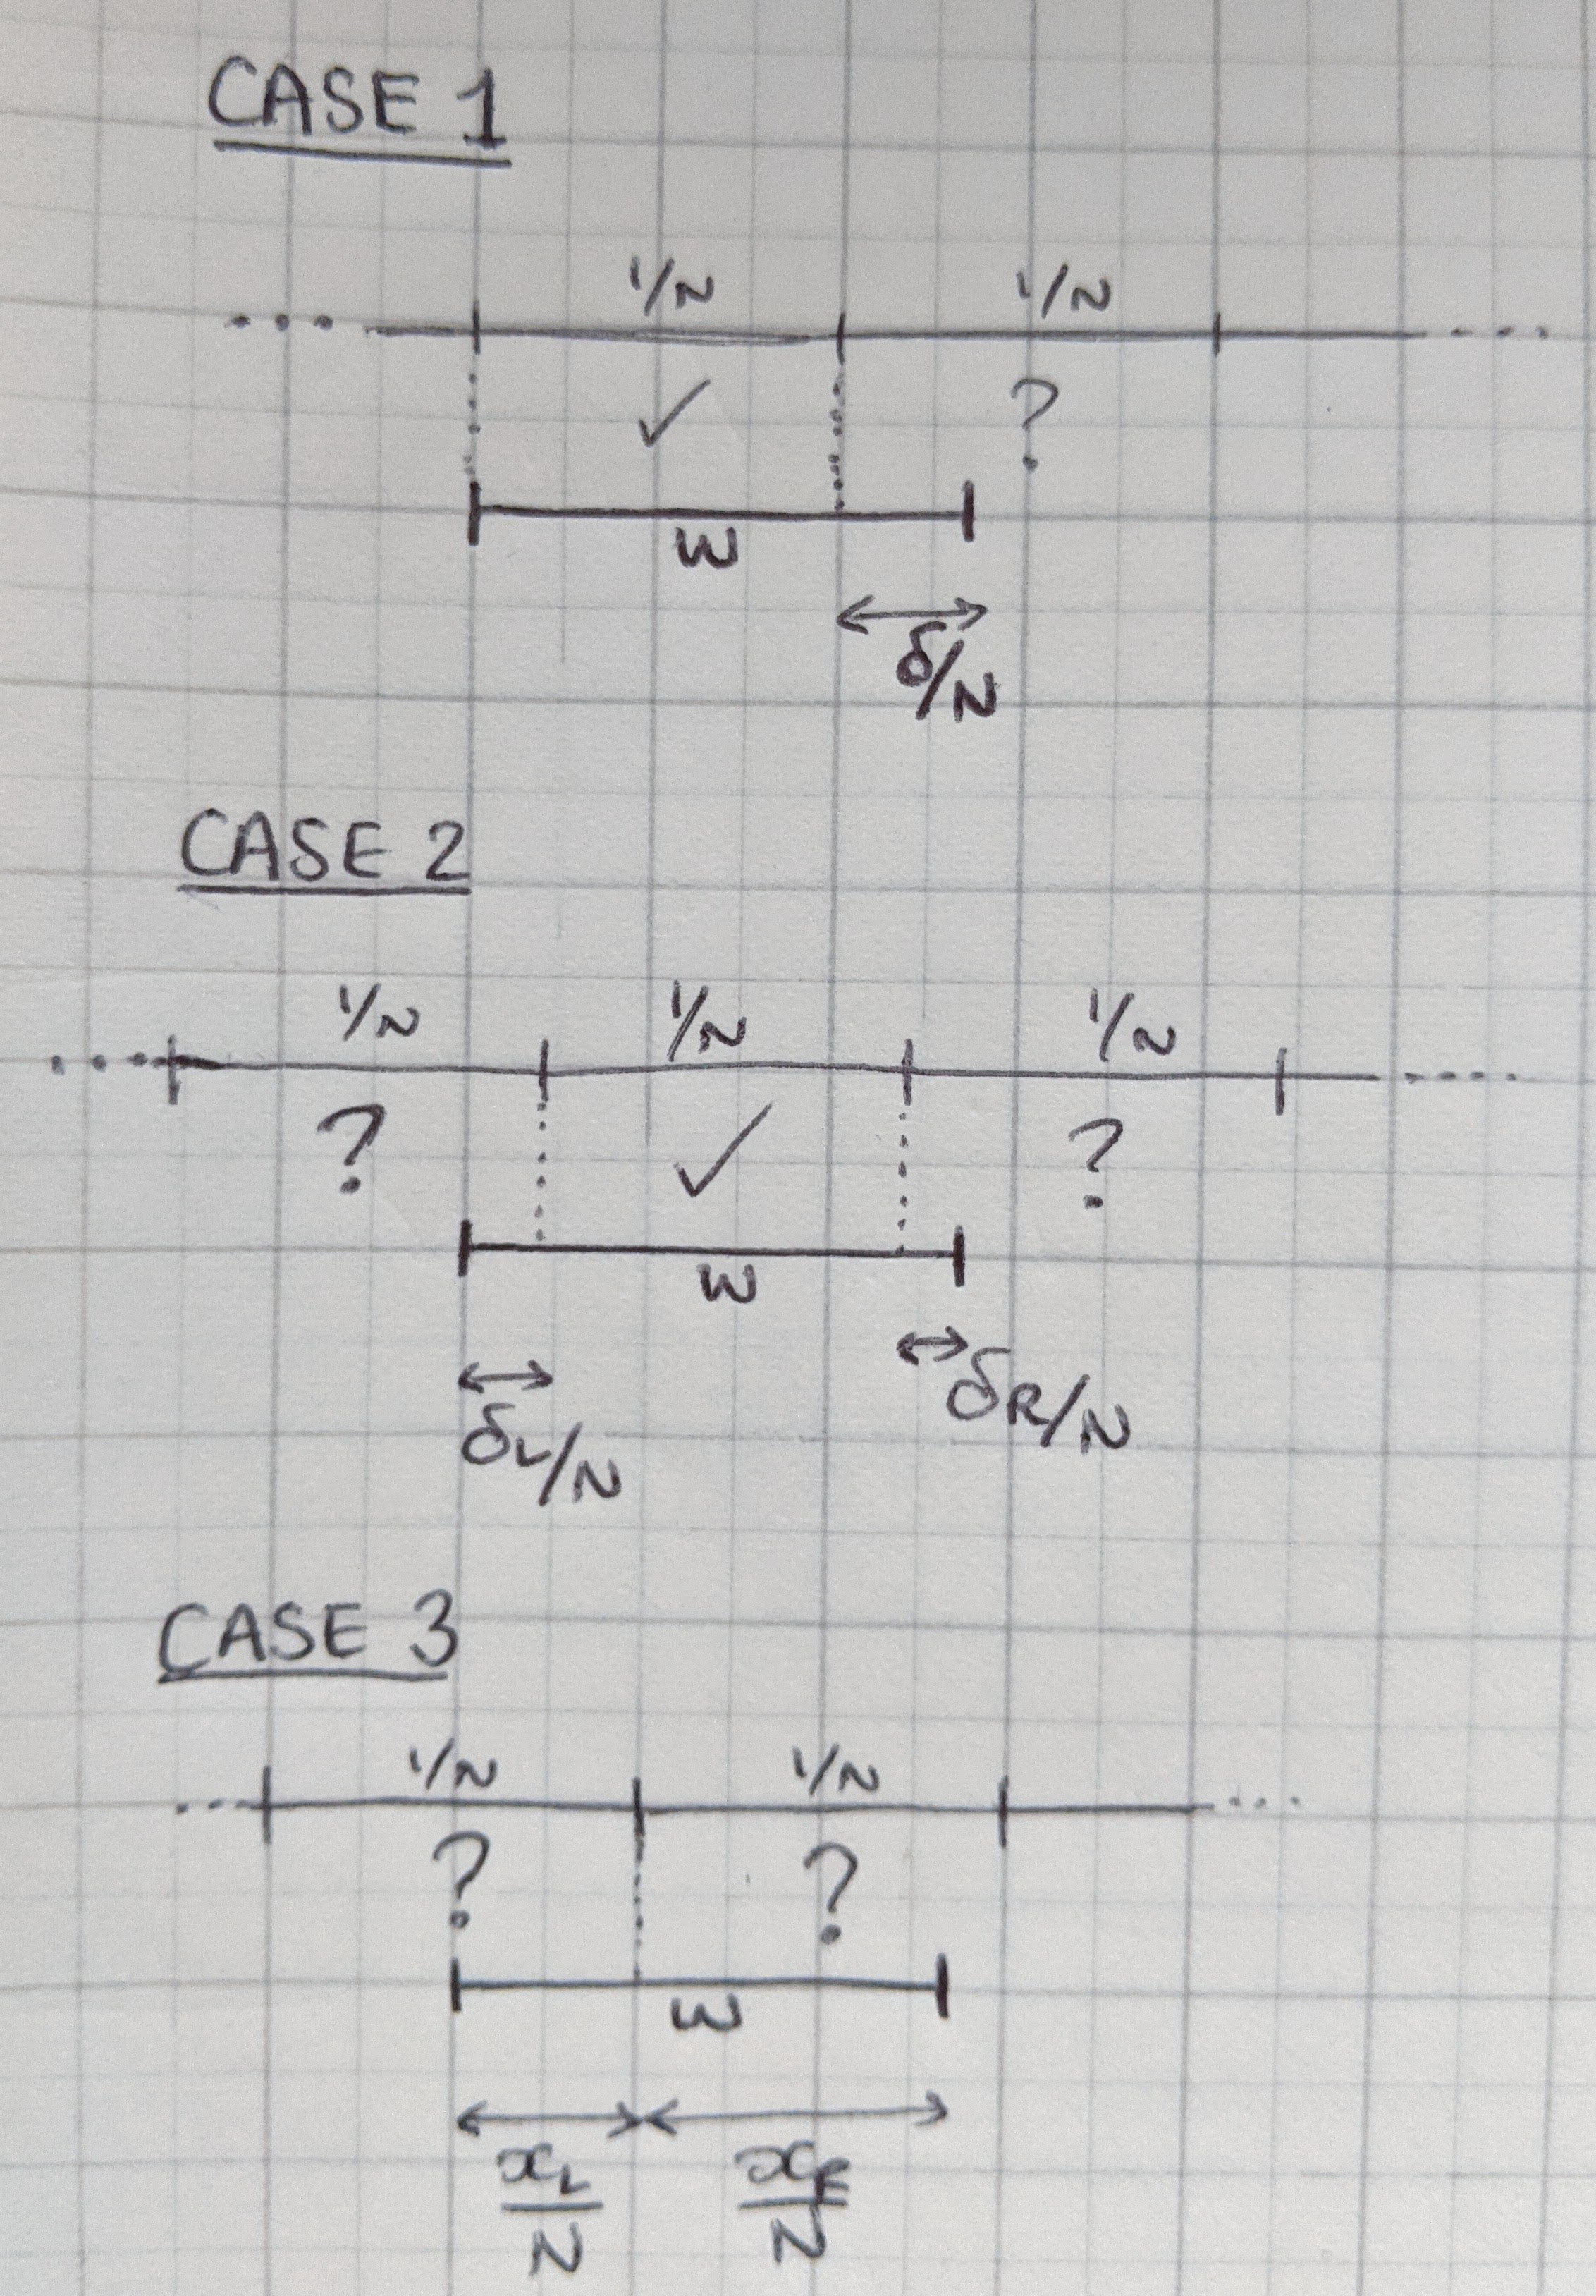
\includegraphics[width=0.4\textwidth]{plots/cases_sketch.jpg}
%\caption[PLACEHOLDER Cases for stratified resampling with a fixed weight]{PLACEHOLDER Cases for stratified resampling with a fixed weight. When I make this properly I need to allow for general $k$ rather than fixing $k=1$ as done here. Case 3 is only valid for $k\geq1$.}
%\label{fig:strat_cases_temp}
%\end{figure}

\begin{figure}
\centering
%\subfloat[Case 1]{
%\begin{tikzpicture}
%% w subinterval
%\draw[thick] (0,0)--(1.9,0);
%\draw[thick,dotted] (1.9,0)--(2.3,0);
%\draw[thick] (2.3,0)--(4.8,0);
%\draw[thick] (0,0.1)--(0,-0.1);
%\draw[thick] (4.8,0.1)--(4.8,-0.1);
%\node[anchor=north] at (2.4,0) {$w$};
%% length labels
%\draw[<->] (0,-0.4)--(4,-0.4);
%\node[anchor=north] at (2,-0.4) {$k/N$};
%\draw[<->] (4,-0.4)--(4.8,-0.4);
%\node[anchor=north] at (4.4,-0.4) {$\delta/N$};
%% sampling interval
%\draw (-0.5,1.5)--(8.5,1.5);
%\draw[dotted] (-1,1.5)--(-0.5,1.5);
%\draw[dotted] (8.5,1.5)--(9,1.5);
%\draw (0,1.6)--(0,1.4);
%\draw (4,1.6)--(4,1.4);
%\draw (8,1.6)--(8,1.4);
%\node[anchor=south] at (2,1.5) {$k/N$};
%\node[anchor=south] at (6,1.5) {$1/N$};
%% vertical dividers
%\draw[dashed, gray] (0,1.4)--(0,0.1);
%\draw[dashed, gray] (4,1.4)--(4,0.1);
%\end{tikzpicture}
%}\\
\subfloat[The parent under consideration is automatically assigned $k$ offspring, plus up to two more. ($\delta_L+\delta_R=\delta$.)]{
\begin{tikzpicture}
% w subinterval
\draw[thick] (0,0)--(1.9,0);
\draw[thick,dotted] (1.9,0)--(2.3,0);
\draw[thick] (2.3,0)--(4.8,0);
\draw[thick] (0,0.1)--(0,-0.1);
\draw[thick] (4.8,0.1)--(4.8,-0.1);
\node[anchor=north] at (2.4,0) {$w$};
% length labels
\draw[<->] (0.3,-0.4)--(4.3,-0.4);
\node[anchor=north] at (2,-0.4) {$k/N$};
\draw[<->] (4.3,-0.4)--(4.8,-0.4);
\node[anchor=north] at (4.55,-0.4) {$\delta_R/N$};
\draw[<->] (0,-0.4)--(0.3,-0.4);
\node[anchor=north] at (0.15,-0.4) {$\delta_L/N$};
% sampling interval
\draw (-4.2,1.5)--(8.8,1.5);
\draw[dotted] (-4.7,1.5)--(-4.2,1.5);
\draw[dotted] (8.8,1.5)--(9.3,1.5);
\draw (-3.7,1.6)--(-3.7,1.4);
\draw (0.3,1.6)--(0.3,1.4);
\draw (4.3,1.6)--(4.3,1.4);
\draw (8.3,1.6)--(8.3,1.4);
\node[anchor=south] at (-1.7,1.5) {$1/N$};
\node[anchor=south] at (2.3,1.5) {$k/N$};
\node[anchor=south] at (6.3,1.5) {$1/N$};
% vertical dividers
\draw[dashed, gray] (0.3,1.4)--(0.3,0.1);
\draw[dashed, gray] (4.3,1.4)--(4.3,0.1);
\end{tikzpicture}
\label{fig:strat_case1}
}\\
\subfloat[This case can only occur when $k\geq1$. The parent under consideration is automatically assigned $k-1$ offspring, plus up to two more. ($x_L+x_R=1+\delta$.)]{
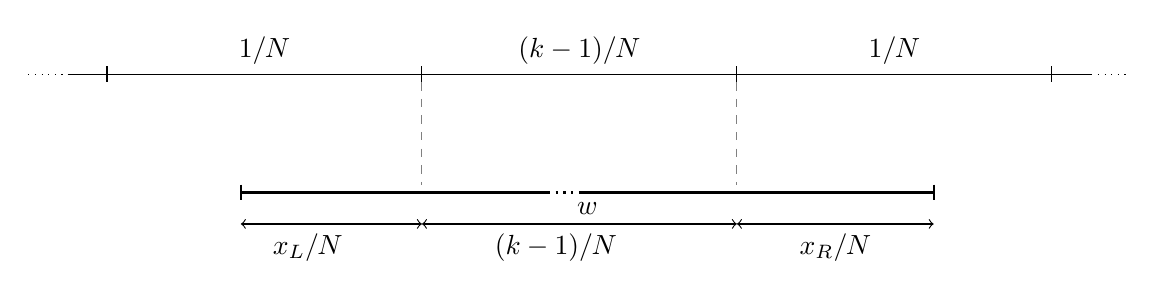
\begin{tikzpicture}
% w subinterval
\draw[thick] (-2,0)--(1.9,0);
\draw[thick,dotted] (1.9,0)--(2.3,0);
\draw[thick] (2.3,0)--(6.8,0);
\draw[thick] (-2,0.1)--(-2,-0.1);
\draw[thick] (6.8,0.1)--(6.8,-0.1);
\node[anchor=north] at (2.4,0) {$w$};
% length labels
\draw[<->] (0.3,-0.4)--(4.3,-0.4);
\node[anchor=north] at (2,-0.4) {$(k-1)/N$};
\draw[<->] (4.3,-0.4)--(6.8,-0.4);
\node[anchor=north] at (5.55,-0.4) {$x_R/N$};
\draw[<->] (-2,-0.4)--(0.3,-0.4);
\node[anchor=north] at (-1.15,-0.4) {$x_L/N$};
% sampling interval
\draw (-4.2,1.5)--(8.8,1.5);
\draw[dotted] (-4.7,1.5)--(-4.2,1.5);
\draw[dotted] (8.8,1.5)--(9.3,1.5);
\draw (-3.7,1.6)--(-3.7,1.4);
\draw (0.3,1.6)--(0.3,1.4);
\draw (4.3,1.6)--(4.3,1.4);
\draw (8.3,1.6)--(8.3,1.4);
\node[anchor=south] at (-1.7,1.5) {$1/N$};
\node[anchor=south] at (2.3,1.5) {$(k-1)/N$};
\node[anchor=south] at (6.3,1.5) {$1/N$};
% vertical dividers
\draw[dashed, gray] (0.3,1.4)--(0.3,0.1);
\draw[dashed, gray] (4.3,1.4)--(4.3,0.1);
\end{tikzpicture}
\label{fig:strat_case2}
}
\caption[Cases for stratified resampling with a fixed weight]{Cases for stratified resampling with a fixed weight}
\label{fig:strat_cases}
\end{figure}


In any case $\nu_t^{(i)} \in \{k-1,k,k+1,k+2\}$ almost surely. 
To define a probability distribution over these four values, we introduce the notation $p_j := \Prob[ \nu_t^{(i)} = \flnw +j \mid w_t^{(i)} ]$, for $j=-1,0,1,2$. 
Since the sample within each interval of length $1/N$ is uniform over that interval, we find the probabilities given in Table~\ref{tab:strat_probs}, in terms of $\delta$ and the other quantities $\delta_L, \delta_R, x_L, x_R$ defined in Figure~\ref{fig:strat_cases}. The probabilities do not depend on $k$, but of course the corresponding values of $\nu_t^{(i)}$ do. By definition $\delta_L+\delta_R=\delta$ and $x_L+x_R=1+\delta$.

\begin{table}[ht]
\centering
\begin{tabular}{ c | c c }
\hline\hline
& Case \subref{fig:strat_case1} & Case \subref{fig:strat_case2}\\
\hline
$p_{-1}$ & 0 & $x_Lx_R-\delta$\\
$p_0$ & $1-\delta + \delta_L\delta_R$ & $1+\delta-2x_Lx_R$\\
$p_1$ & $\delta-2\delta_L\delta_R$ & $x_Lx_R$\\
$p_2$ & $\delta_L\delta_R$ & 0\\
\hline\hline
\end{tabular}
\caption[Analysis of distribution of offspring counts under stratified resampling]{Marginal probability distribution of $\nu_t^{(i)}$ conditional on $w_t^{(i)}$, in terms of $\delta$ and the quantities defined in Figure~\ref{fig:strat_cases}.}
\label{tab:strat_probs}
\end{table}

By considering the constraints on $\delta_L, \delta_R, x_L, x_R$, we also have the following properties which hold in every case (i.e.\ for any $w_t^{(i)}$):
\begin{itemize}
\item $p_{-1} \leq 1/4$
\item $p_{2} \leq 1/4$
\item only one of $p_{-1}, p_2$ can be non-zero.
\end{itemize}




\subsubsection{Systematic resampling \seb{$\checkmark$} }%\label{sec:resampling_systematic}
Systematic resampling is described in \textcite{carpenter1999} and also in \textcite{whitley1994} where it is called ``stochastic universal sampling''.

Like stratified resampling, it uses the inversion sampler of multinomial resampling but starts with a more regular set of points in $[0,1]$.
In this scheme, only one standard Uniform sample is drawn, $u \sim \Unif[0,1]$, from which the $N$ samples are generated by via the transformation
\begin{equation*}
U_i = \frac{u+ i-1}{N}
\end{equation*}
for $i = 1, \dots, N $.
The parental indices are again selected according to \eqref{eq:syst_strat_resampling}. 
The method is illustrated in Figure \ref{fig:resampling_systematic}.

\textcite{kitagawa1996} suggests a deterministic scheme in which the random $u$ is replaced by a fixed $\alpha\in[0,1]$; but, being deterministic, this scheme does not satisfy the unbiasedness property (condition~\ref{item:resampling_property1} in Definition~\ref{defn:resampling}).
\textcite{whitley1994} describes systematic resampling using a different picture, whereby the interval $[0,1]$ is joined up into a circle, and the systematic samples are evenly spaced pointers on an outer ring, which is spun around like a roulette wheel to sample a random phase which, modulo 1, is equal to $u$.\seb{figure please}
For systematic resampling, Whitley's ``roulette wheel'' representation is equivalent to that of Figure~\ref{fig:resampling_systematic}.

Like stratified resampling, systematic resampling ensures the random numbers are ``well spread out''; the resulting samples are even more constrained than with stratified resampling. 
Systematic resampling also has the advantage of being extremely easy to implement and also computationally efficient, requiring only one sample from a pseudo-random number generator (PRNG) followed by $O(N)$ elementary operations.

However, this scheme is known to exhibit pathological behaviour in some cases because its performance depends on the ordering of the weights. A simple example of this phenomenon is presented in \textcite{douc2005}. 
Such behaviour can be avoided by randomly permuting the weights before resampling, and this is the recommended practice. 



\subsubsection{Star resampling \seb{$\checkmark$} }%\label{sec:resampling_star}
For the sake of comparison, we also construct a resampling scheme which is the worst possible (in some sense).
Sample
\begin{equation*}
a_t \sim \Cat( \{1,\dots, N\}, w_t^{(1:N)} )
\end{equation*}
and set $a_t^{(i)} = a_t$ for all $i$.
The resulting offspring counts are all equal to zero except for $\nu_t^{(a_t)}$, which is equal to $N$.
This resampling scheme is indeed unbiased, since each offspring count has marginal distribution
\begin{equation*}
\nu_t^{(i)}  \mid w_t^{(1:N)} 
= \begin{cases}
0 & \text{w.p. } 1-w_t^{(i)} \\
N & \text{w.p. } w_t^{(i)} .
\end{cases}
\end{equation*}
We also see these offspring counts have the highest possible marginal variance, subject to $\E[ \nu_t^{(i)}  \mid w_t^{(i)} ] = Nw_t^{(i)}$ and $\nu_t^{(i)} \in \{0,\dots,N\}$.

I call this scheme \emph{star resampling} because the parent-offspring relationships at each iteration form a star graph.


\subsubsection{Minimum-variance resampling}

The minimal variance branching algorithm of \textcite{crisan1999} provides a framework for minimal-variance resampling. The idea is to enforce minimal variance by resampling such that each offspring count $\nu_t^{(i)}$, conditionally on $w_t^{(i)}$, has marginal distribution
\begin{equation}\label{eq:branching_distn}
\nu_t^{(i)} \mid w_t^{(i)} \eqdist \flnw + \Bern(Nw_t^{(i)} - \flnw) .
\end{equation}
We will see later on that this is exactly the framework of \emph{stochastic rounding}.
The set-up of \textcite{crisan1999} does not require the number of particles to remain constant from one generation to the next (Property~\ref{item:resampling_property1} in Definition~\ref{defn:resampling}), so their minimal variance branching algorithm could be implemented for instance by sampling each $\nu_t^{(i)}$ independently from \eqref{eq:branching_distn}. The authors remark that enforcing strictly negative correlation between the offspring counts can improve the rate of convergence, but they do not specify how this might be achieved.

\draft{Also write about \textcite{gerber2017}, which in some sense extends/formalises the notions of \textcite{crisan1999}.}




\subsection{Properties \seb{$\sim$} }\label{sec:resampling_properties}
\draft{Low-variance: variance of what? Different criteria/ definitions of optimality. Link back to adaptive resampling: interaction between adaptive and low-variance resampling. Comparison of properties of these, existing results comparing schemes. Implementation considerations. Theoretical justification (or lack of). Mention computational complexity.}
\seb{This section was dumped from elsewhere and most of its subsections need redrafting. Also add a paragraph here to introduce it, saying that everything is summarised in the table.}



\subsubsection{Support of offspring numbers \seb{$\checkmark$} }
Let us consider the support of the marginal offspring distributions in each scheme, conditional on the weights. Suppose that the $i^{th}$ weight lies in the interval $w_t^{(i)} \in [k/N, (k+1)/N]$.

Under multinomial resampling, it is possible for $\nu_t^{(i)}$ to take any value from $0$ to $N$ (although some values are of course more likely than others).
Thus it is possible for a high-weight particle to have zero offspring, or a low-weight particle to have many offspring, simply by chance.
Recall that the weights give an indication of how ``useful'' each particle is for the approximation. Thus killing a high-weight particle is likely to increase the variance of the SMC estimates, while duplicating a low-weight particle wastes computational resources on propagating particles that will not contribute much to reducing that variance.

Residual resampling ensures that every particle with above-average (i.e.\ $>1/N$) weight has at least one offspring, avoiding the loss of high-weight particles. If the residuals are sampled using multinomial resampling then the duplication of low-weight particles is not avoided, $\nu_t^{(i)} \in \{k, \dots, k+R\} \subseteq \{k,\dots, N\}$, but this can be addressed by using a lower-variance scheme for the residual offspring. Various choices are included in Table~\ref{tab:resampling_properties}.

Stratified resampling is more restrictive, $\nu_t^{(i)} \in \{k-1, k, k+1, k+2\}$, but allows the possibility of a particle with above-average weight having no offspring. 
Systematic resampling has the smallest support, $\nu_t^{(i)} \in \{k, k+1\}$, that is possible whilst maintaining unbiasedness.

Another way to quantify this property is by considering the maximum possible difference between the offspring count $\nu_t^{(i)}$ and its expected value $N w_t^{(i)}$. This is also presented in Table~\ref{tab:resampling_properties}.




\subsubsection{Degeneracy under equal weights \seb{$\checkmark$} }
In the case where all of the weights are multiples of $1/N$, low-variance schemes such as residual and systematic resampling become fully deterministic. 
Since $\flnw = Nw_t^{(i)}$ for each $i$, residual resampling will have $R=0$ leaving no remainder to be assigned stochastically. 
In systematic resampling exactly $\flnw = Nw_t^{(i)}$ samples will fall in the $i^{th}$ interval.
In particular, if $w_t^{(1:N)} = (1,\dots, 1)/N$ then each parent is assigned exactly one offspring deterministcially, so there is effectively no resampling.

The same phenomenon occurs with stratified resampling, but not if one uses Whitley's roulette wheel description\seb{(Figure ??)}. The random phase shift introduced by ``spinning the wheel'' prevents the inversion sampling intervals from lining up exactly with the weight intervals, so the resampled offspring counts may vary from their means by one either side.
\textcite{whitley1994} does not describe stratified resampling, but we see that unlike with systematic resampling, the roulette wheel description is not equivalent to the standard inversion sampling description. 
For stratified resampling, the roulette wheel adds some extra randomness, so the straightforward inversion sampler is preferred.

If the state space is continuous, the event that all weights are multiples of $1/N$ typically has zero measure, but with non-zero probability we can get arbitrarily close to this regime in which resampling becomes deterministic.




\subsubsection{Marginal variance of offspring counts \seb{$\checkmark$} }
\draft{Mention negative association? $=$ teaser for later, which has to do with covariance between counts rather than marginal variance.}

One indication of the performance could be the variance of the resampled offspring counts. For instance we might ask what is the marginal variance of $\nu_t^{(i)}$, conditional on the corresponding weight $w_t^{(i)}$.

In multinomial resampling, the marginal distributions are
\begin{equation*}
\nu_t^{(i)} \mid w_t^{(i)} 
\sim \Bin(N, w_t^{(i)})
\end{equation*}
so the variance is
\begin{equation*}
\V[ \nu_t^{(i)} \mid w_t^{(i)} ]
= N w_t^{(i)} ( 1- w_t^{(i)} ) .
\end{equation*}
Compare this to star resampling, where the marginal offspring counts
\begin{equation*}
\nu_t^{(i)} \mid w_t^{(i)} 
\eqdist N \Bern( w_t^{(i)} )
\end{equation*}
having variance
\begin{equation*}
\V[ \nu_t^{(i)} \mid w_t^{(i)} ]
= N^2 w_t^{(i)} ( 1- w_t^{(i)} ) ,
\end{equation*}
$N$ times larger than in the multinomial case.

As pointed out in \textcite[p.557]{crisan1999}, their minimal variance branching process yields offspring variance
\begin{equation*}
\V[ \nu_t^{(i)} \mid w_t^{(i)} ]
= ( Nw_t^{(i)} -\flnw )(1- Nw_t^{(i)} + \flnw) 
\leq \frac{1}{4} ,
\end{equation*}
since the stochastic part of $\nu_t^{(i)}$ is a $\Bern( Nw_t^{(i)} -\flnw )$ random variable (as seen in \eqref{eq:branching_distn}).
The same marginal variance appears from systematic, residual-systematic and SSP resampling, since these all share the same marginal offspring distributions. We will see in Section~\ref{sec:SRs} that all of these schemes fall within the \emph{stochastic rounding} class, and the marginal offspring variance is a property shared by all stochastic roundings.

The marginal variance is harder to calculate for other schemes such as residual-multinomial and stratified resampling because these were not defined in terms of marginal distributions, nor are the offspring counts independent conditional on the weights.
However, it is possible in some cases to find upper bounds on the variance, and some such bounds are derived below.

Residual-multinomial: $\nu_t^{(i)}$ depends on all of the other weights, as well as $w_t^{(i)}$, but only through the statistic $R := \sum (N w_t^{(i)} - \flnw)$.
We have
\begin{equation*}
\nu_t^{(i)} \mid w_t^{(i)} , R
\eqdist \flnw + \Bin\left( R, \frac{Nw_t^{(i)} - \flnw}{R} \right) .
\end{equation*}
Using the law of total variance,
\begin{align*}
\V[ \nu_t^{(i)} \mid w_t^{(i)} ]
&= \E\left[ \V[ \nu_t^{(i)} \mid w_t^{(i)}, R ] \mid w_t^{(i)} \right]
        + \V\left[ \E[ \nu_t^{(i)} \mid w_t^{(i)}, R ] \mid w_t^{(i)} \right] \\
&= \E\left[ (Nw_t^{(i)} - \flnw) \left( 1- \frac{Nw_t^{(i)} - \flnw}{R} \right) 
        \mid w_t^{(i)} \right] \\
    &\qquad+ \V\left[ Nw_t^{(i)} \mid w_t^{(i)} \right] \\
&= Nw_t^{(i)} - \flnw - (Nw_t^{(i)} - \flnw)^2\, \E[ R^{-1} \mid w_t^{(i)} ] \\
% &\leq \E\left[ Nw_t^{(i)} - \flnw \mid w_t^{(i)} \right]
%        + \V\left[ Nw_t^{(i)} \mid w_t^{(i)} \right] \\
&\leq Nw_t^{(i)} - \flnw .
\end{align*}
Similarly, for residual resampling with star residuals,
\begin{equation*}
\nu_t^{(i)} \mid w_t^{(i)} , R
\eqdist \flnw + R \Bern\left( \frac{Nw_t^{(i)} - \flnw}{R} \right) .
\end{equation*}
and we find
\begin{align*}
\V[ \nu_t^{(i)} \mid w_t^{(i)} ]
&= \E\left[ \V[ \nu_t^{(i)} \mid w_t^{(i)}, R ] \mid w_t^{(i)} \right]
        + \V\left[ \E[ \nu_t^{(i)} \mid w_t^{(i)}, R ] \mid w_t^{(i)} \right] \\
&= \E\left[ R (Nw_t^{(i)} - \flnw) \left( 1- \frac{Nw_t^{(i)} - \flnw}{R} \right) 
        \mid w_t^{(i)} \right] \\
    &\qquad+ \V\left[ Nw_t^{(i)} \mid w_t^{(i)} \right] \\
&= \E\left[ R (Nw_t^{(i)} - \flnw) \left( 1- \frac{Nw_t^{(i)} - \flnw}{R} \right) 
        \mid w_t^{(i)} \right] \\
&= (Nw_t^{(i)} - \flnw) \E\left[ R \mid w_t^{(i)} \right]  - (Nw_t^{(i)} - \flnw)^2 \\
&\leq N (Nw_t^{(i)} - \flnw) .
\end{align*}

For stratified resampling, we can use the constraints on the marginal offspring distribution that were derived in Section~\ref{sec:examples_resamplingschemes}. Recall that, conditional on $w_t^{(i)}$, $\nu_t^{(i)} = \flnw + j$ with probability $p_{j}$ for $j=-1,0,1,2$.
We can use the values of $p_{-1},p_0,p_1,p_2$ in the two cases of Figure~\ref{fig:strat_cases}, as summarised in Table~\ref{tab:strat_probs}, to bound the variance. First write
\begin{align*}
\V[ \nu_t^{(i)} \mid w_t^{(i)} ]
&= \E[ (\nu_t^{(i)} - \flnw)^2 \mid w_t^{(i)} ] 
        - \E[ \nu_t^{(i)} -\flnw \mid w_t^{(i)} ]^2 \\
&= p_{-1} + p_1 + 4p_2 - (-p_{-1} + p_1 + 2p_2)^2 .
%\leq 1/2 .
\end{align*}
In Case~\subref{fig:strat_case1}, we have
\begin{equation*}
\V[ \nu_t^{(i)} \mid w_t^{(i)} ]
= (\delta -2\delta_L\delta_R + 4\delta_L\delta_R) 
        - (\delta - 2\delta_L\delta_R + 2\delta_L\delta_R)^2
= \delta +2\delta_L\delta_R - \delta^2
\end{equation*}
which is maximised at $\delta_L=\delta_R=\delta/2$ for a maximum variance of $\delta(1-\delta/2)$, which is at most $1/2$.
In Case~\subref{fig:strat_case2}, we have
\begin{equation*}
\V[ \nu_t^{(i)} \mid w_t^{(i)} ]
= (x_Lx_R -\delta + x_Lx_R) - (-x_Lx_R + \delta + x_Lx_R)^2
= \delta + 2x_Lx_R -\delta^2
\end{equation*}
which is maximised at $x_L=x_R=(1+\delta)/2$ for a maximum variance of $(1-\delta^2)/2$, which is at most $1/2$.
Overall we have the bound
\begin{equation*}
\V[ \nu_t^{(i)} \mid w_t^{(i)} ]
\leq \frac{1}{2}
\end{equation*}
for any $w_t^{(1:N)}$.

Residual-stratified resampling has the further constraint that $p_{-1} =0$ (i.e.\ Case 3 of Figure~\ref{fig:strat_cases} doesn't occur) since the residual weights are between $0$ and $1/R$. However this does not give an improvement on the stratified bound:
\begin{equation*}
\V[ \nu_t^{(i)} \mid w_t^{(i)} ] \leq 1/2 .
\end{equation*}

Table~\ref{tab:resampling_properties} includes upper bounds on $\V[\nu_t^{(i)}]$ for various resampling schemes, independent of $w_t^{(i)}$. Those general bounds are derived from the results of this section, bounded above independently of the weights. Some of the bounds are certainly not tight.




\subsubsection{Contribution to the Monte Carlo variance}
\draft{Finish the proof. Remark that we can't do a formal variance comparison for syst (and others?).}

While the variance of the offspring counts goes some way to providing a comparison between the various resampling schemes, a more relevant property is the contribution of the resampling step to the Monte Carlo variance.
This quantifies directly the effect that a certain choice of resampling scheme has on the variance of the Monte Carlo estimators.

Let $(\mathcal{G}_t)_{t\geq0}$ be the filtration generated by the particle positions and weights up to and including time $t$.
Let $\tilde{X}_t^{(i)}$ denote position of the $i$th resampled particle.
We consider the one-step Monte Carlo variance induced by resampling, that is
\begin{equation}\label{eq:resamplingMCvariance}
\rho(\varphi) 
:= \V\left[ \frac{1}{N} \sum_{i=1}^N \varphi (\tilde{X}_t^{(i)}) \midd \mathcal{G}_t \right]
\end{equation}
where $\varphi$ is an arbitrary test function.

Some results comparing this variance across different resampling schemes are presented in \textcite{douc2005}. 
Their results, plus some additional results, are presented in Proposition~\ref{thm:resampling_var_compare}.

\begin{prop}[Variance of resampling schemes]\label{thm:resampling_var_compare}
Let $\rho_{\texttt{multi}}$ etc.\ denote the variance \eqref{eq:resamplingMCvariance} under the various resampling schemes, as abbreviated in Table~\ref{tab:resampling_abbrevs}.
For any square-integrable\seb{?} function $\varphi$,
\begin{enumerate}[label=(\alph*)]
\item \label{item:resampling_var1} \hspace{5pt}
$\begin{aligned}
    \rho_{\texttt{multi}}(\varphi) 
    \geq \rho_{\texttt{res-multi}}(\varphi)
\end{aligned}$
\item \label{item:resampling_var2} \hspace{5pt}
$\begin{aligned}
    \rho_{\texttt{multi}}(\varphi) 
    \geq \rho_{\texttt{strat}}(\varphi)
\end{aligned}$
\item \label{item:resampling_var3} \hspace{5pt}
$\begin{aligned}
    \rho_{\texttt{star}}(\varphi) 
    = N \rho_{\texttt{multi}}(\varphi)
\end{aligned}$
\item \label{item:resampling_var4} \hspace{5pt}
$\begin{aligned}
    \rho_{\texttt{res-star}}(\varphi) 
    \geq \rho_{\texttt{res-multi}}(\varphi) 
    \geq \rho_{\texttt{res-strat}}(\varphi)
\end{aligned}$
\end{enumerate}
\end{prop}
Parts \ref{item:resampling_var1} and \ref{item:resampling_var2} were proved in \textcite[Section 3]{douc2005}. The second inequality in \ref{item:resampling_var4} is stated in \textcite[p.9]{gerber2017} and follows from \ref{item:resampling_var2}, as shown below.

\begin{proof}
\textbf{multinomial resampling:} the resampled indices are conditionally i.i.d., so
\begin{align*}
\rho_{\texttt{multi}}(\varphi)
&= \V\left[ \frac{1}{N} \sum_{i=1}^N \varphi (\tilde{X}_t^{(i)}) 
        \midd \mathcal{G}_t \right]
= \frac{1}{N} \V\left[ \varphi (\tilde{X}_t^{(i)}) 
        \midd \mathcal{G}_t \right] \\
&= \frac{1}{N} \left\{ \E\left[ \varphi^2(\tilde{X}_t^{(i)}) \midd \mathcal{G}_t \right]
        - \E\left[ \varphi(\tilde{X}_t^{(i)}) \midd \mathcal{G}_t \right]^2 \right\} \\
&= \frac{1}{N} \sum_{j=1}^N \varphi^2(X_t^{(j)}) 
        \Prob[\tilde{X}_t^{(i)} = X_t^{(j)} \mid \mathcal{G}_t ]
        - \frac{1}{N} \left\{ \sum_{j=1}^N \varphi(X_t^{(j)}) 
        \Prob[\tilde{X}_t^{(i)} = X_t^{(j)} \mid \mathcal{G}_t ] \right\}^2 \\
&= \frac{1}{N} \sum_{j=1}^N \varphi^2(X_t^{(j)}) w_t^{(j)}
        - \frac{1}{N} \left\{ \sum_{j=1}^N \varphi(X_t^{(j)}) w_t^{(j)} \right\}^2 .        
\end{align*}

\textbf{star resampling:} all of the resampled indices are equal, say $\tilde{X}_t^{(1)} = \dots = \tilde{X}_t^{(N)} = X_t^\star$, so
\begin{align*}
\rho_{\texttt{star}}(\varphi)
&= \V\left[ \frac{1}{N} \sum_{i=1}^N \varphi(\tilde{X}_t^{(i)}) \midd \mathcal{G}_t \right]
= \V\left[ \varphi( X_t^\star) \mid \mathcal{G}_t \right] \\
&= \E\left[ \varphi^2( X_t^\star) \mid \mathcal{G}_t \right]
        - \E\left[ \varphi( X_t^\star) \mid \mathcal{G}_t \right]^2 \\
&= \sum_{j=1}^N \varphi^2(X_t^{(j)}) 
        \Prob[ X_t^\star = X_t^{(j)} \mid \mathcal{G}_t ]
        - \left\{ \sum_{j=1}^N \varphi(X_t^{(j)}) 
        \Prob[ X_t^\star = X_t^{(j)} \mid \mathcal{G}_t ] \right\}^2 \\
&= \sum_{j=1}^N \varphi^2(X_t^{(j)}) w_t^{(j)}
        - \left\{ \sum_{j=1}^N \varphi(X_t^{(j)}) w_t^{(j)} \right\}^2 \\
&= N \rho_{\texttt{multi}}(\varphi) .
\end{align*}
 This proves part \ref{item:resampling_var3}. Here we see the same factor of $N$ as we had with the marginal variance of offspring counts, due to the variance reduction achieved by taking $N$ independent copies (multinomial resampling) as opposed to $N$ identical copies (star resampling).

\textbf{residual-multinomial resampling:} the Monte Carlo estimate in \eqref{eq:resamplingMCvariance} can be decomposed into a sum of conditionally deterministic terms plus a sum of conditionally i.i.d. terms: conditional on $\mathcal{G}_t$,
\begin{equation*}
\frac{1}{N} \sum_{i=1}^N \varphi (\tilde{X}_t^{(i)})
= \frac{1}{N} \sum_{i=1}^N \flnw \varphi (X_t^{(i)})
        + \frac{1}{N} \sum_{i=1}^R \varphi (\hat{X}_t^{(i)})
\end{equation*}
where
$ \hat{X}_t^{(i)} \sim^{\text{iid}} \Mn( R, r^{(1:N)} ) $.
The first sum is conditionally deterministic and hence does not contribute to the Monte Carlo variance \eqref{eq:resamplingMCvariance}. By a similar calculation to that for multinomial resampling,
\begin{align*}
\rho_{\texttt{res-multi}}(\varphi)
&= \V\left[ \frac{1}{N} \sum_{i=1}^R \varphi (\hat{X}_t^{(i)}) 
        \midd \mathcal{G}_t \right] \\
&= \frac{R}{N^2} \sum_{j=1}^N \varphi^2(X_t^{(j)}) r^{(j)}
        - \frac{R}{N^2} \left( \sum_{j=1}^N \varphi(X_t^{(j)}) r^{(j)} \right)^2 \\
&= \frac{1}{N} \sum_{j=1}^N \varphi^2(X_t^{(j)}) w_t^{(j)}
        - \frac{1}{N^2} \sum_{j=1}^N \varphi^2(X_t^{(j)}) \flnw[j]
        - \frac{R}{N^2} \left( \sum_{j=1}^N \varphi(X_t^{(j)}) r^{(j)} \right)^2 . 
\end{align*}
By a similar argument, it can be shown that
\begin{equation*}
\rho_{\texttt{res-star}}(\varphi)
= R \,\rho_{\texttt{res-multi}}(\varphi)
\geq \rho_{\texttt{res-multi}}(\varphi) ,
\end{equation*}
whenever $R\geq 1$, proving the first inequality in \ref{item:resampling_var4} (which holds trivially when $R=0$ because both residual schemes then have zero variance). \seb{Maybe I should do res-star explicitly actually; if I'm including proofs that have already been published then I ought to include proofs that haven't.}
To prove \ref{item:resampling_var1}, write
\begin{align*}
\rho_{\texttt{res-multi}}(\varphi)
&= \frac{1}{N} \sum_{j=1}^N \varphi^2(X_t^{(j)}) w_t^{(j)}
        - \frac{1}{N} \left\{ \frac{1}{N} \sum_{j=1}^N \varphi^2(X_t^{(j)}) \flnw[j]
        + \frac{R}{N} \left( \sum_{j=1}^N \varphi(X_t^{(j)}) r^{(j)} \right)^2
        \right\} \\
&\leq \frac{1}{N} \sum_{j=1}^N \varphi(X_t^{(j)}) w_t^{(j)}
        - \frac{1}{N} \left\{ \frac{1}{N} \sum_{j=1}^N \varphi^2(X_t^{(j)}) \flnw[j]
        + \frac{R}{N} \sum_{j=1}^N \varphi(X_t^{(j)}) r^{(j)}
        \right\}^2 \\
&= \frac{1}{N} \sum_{j=1}^N \varphi^2(X_t^{(j)}) w_t^{(j)}
        - \frac{1}{N} \left\{ \sum_{j=1}^N \varphi(X_t^{(j)}) w_t^{(j)} \right\}^2
        = \rho_{\texttt{multi}}(\varphi) .
\end{align*}
The inequality is an application of Jensen's inequality, since
\begin{equation*}
\sum_{j=1}^N \frac{ \flnw[j] }{N} + \frac{R}{N} = 1 .
\end{equation*}



...
\end{proof}




\subsubsection{Exchangeability \seb{$\sim$} }
We will call a resampling scheme exchangeable if the resulting distribution of parental indices is invariant under permutations of the children. To put it another way, each child chooses its parent from the same marginal distribution.

It is clear that multinomial resampling is exchangeable since in this case the parental indices are independent and identically distributed. However the efficient implementation of multinomial sampling that takes sorted inputs does not preserve exchangeability.

Stratified and systematic resampling are clearly not exchangeable since, for instance, child 1 is more likely to choose parent 1 than child $N$ is. However, this is merely a feature of the arbitrary ordering of the sampling steps: exchangeability can easily be reintroduced (at $O(N)$ cost) by applying a random permutation to the vector of parental indices after sampling.
The same goes for residual resampling.
\seb{This property will not appear in Table~\ref{tab:resampling_properties} since it depends upon the particular implementation.}





\subsubsection{Permutation invariance \seb{$\checkmark$} }
A strange property of stratified and systematic resampling is that they are sensitive to the order in which the subintervals are placed. For example, in Figures \ref{fig:resampling_stratified} and \ref{fig:resampling_systematic} if the intervals $w_2$ and $w_4$ were swapped, the number of offspring assigned to particles 2 and 4 would be swapped in each case. \seb{Better to use an example where \emph{distribution} of offspring counts (conditional on the weights but not on the Uniform samples) differs depending on order. Such an example is included in my YRM19 presentation on resampling.}
We can also see that because $w_1$ has weight $\geq 1/N$ and is placed first, it is guaranteed at least one offspring.

This property can lead to pathological behaviour, but is easily avoided by applying a random permutation to the order of the subintervals.
The SSP resampling scheme of \textcite{gerber2017} is intended to share the benefits of systematic resampling whilst avoiding this property.




\subsubsection{Sorting}
\draft{Results from \textcite{gerber2017} about benefits of sorting. What about sorting instead by weights?}



\subsubsection{Computational complexity \seb{$\checkmark$} }
All of the resampling algorithms discussed in Section~\ref{sec:examples_resamplingschemes} can be implemented in $O(N)$ operations.
\seb{Even \texttt{star} and \texttt{SSP} and \texttt{branching}? If it turns out to differ depending on resampling scheme then include it as a column in Table~\ref{tab:resampling_properties}. --- I think we can't say for \texttt{branching} becaue it dpeends on implementation, but \textcite[Corollary 18]{crisan1999} seems to imply $O(N^2)$...? SSP is definitely $O(N)$.}
Considering the complexity of each operation, \textcite{hol2004,hol2006} suggest that systematic resampling is fastest because it only requires one pseudo-random number generation, and multinomial resampling is slower than stratified resampling because of the transformations required. Residual resampling is hard to compare directly because a random fraction of the operations are deterministic, so the number of pseudo-random numbers required is less than $N$.
This analysis was backed up by simulation experiments.
However, the analysis of per-particle cost is sensitive to the particular implementation of each resampling scheme, the system implementation of pseudo-random number generation and arithmetic operations, and the hardware used.




\subsubsection{Negative association}
\draft{Definition from \textcite{gerber2017}. Why is it a good criterion? Which resampling schemes do/don't satisfy it? Also, this could be added as a column in Table~\ref{tab:resampling_properties}.}

Following \textcite{gerber2017}, we use the definition of negative association from \textcite{joag1983}.
\begin{defn}
Let $(Z_1, \dots, Z_n)$ be a collection of random variables. 
$Z_{1:n}$ are said to be \emph{negatively associated} if, for every partition of $\{1,\dots, n\}$ into subsets $I$ and $J$, for all real-valued coordinatewise non-decreasing functions $\varphi, \psi$ for which the covariance is well defined,
\begin{equation*}
\Cov \left[ \varphi( Z_I) , \psi(Z_J) \right] \leq 0 .
\end{equation*}
\end{defn}



\subsubsection{Star discrepancy \seb{$\checkmark$} }
\draft{(See \textcite{hol2006} for inspiration.) Include a diagram showing the quantity inside the $D^\star$ supremum, plotted over $u$, for mn/strat/syst? (sketched in sora --- use same weights and samples as in Figure~\ref{fig:resampling_mn}.)}
\seb{Does not appear in Table~\ref{tab:resampling_properties} since it only makes sense for resampling schemes based on inversion sampling.}
%
%Since resampling can itself be thought of as a Monte Carlo procedure, it is also open to the tools of quasi-Monte Carlo.
%The idea is to use sample points that are more regularly spaced, with the hope that this will reduce the variance of Monte Carlo estimators.

The \emph{star discrepancy}\seb{[citation]} is a measure of the regularity of a given set of points $u_{1:N}$ in the unit hypercube. For our purposes it is sufficient to define the star discrepancy in one dimension:
\begin{equation*}
D^\star (u_1, \dots, u_N) := \sup_{u \in [0,1]} \left| \frac{1}{N} \sum_{i=1}^N \I{u_i \leq u} -u \right| .
\end{equation*}
The quantity inside the supremum is the difference between the empirical CDF of the observed points $u_{1:N}$ and the CDF of the Uniform distribution on $[0,1]$.
%Thus $D^\star$ tells us, in a specific sense, how far our points are from being uniformly spaced.
The star discrepancy is used in quasi-Monte Carlo, where ``low-discrepancy'' points are used in place of uniform samples to decrease the variance of Monte Carlo estimates.

We have noted already \seb{we haven't actually, but we should} that resampling can itself be viewed as a Monte Carlo procedure.
From this point-of-view, stratified and systematic resampling are quasi-Monte Carlo versions of multinomial resampling, since they provide ``more regular'' points to be used in inversion sampling.

In one dimension, the lowest-discrepancy point set is the regular grid $( \frac{1}{2N}, \frac{3}{2N}, \dots, \frac{2N-1}{2N} )$, which has star discrepancy $1/(2N)$ \seb{[citation]}.
However, to maintain unbiasedness of resampling, the points must have marginal $\Unif[0,1]$ distributions\seb{erm, they don't in e.g.\ strat and syst. what is the actual requirement?}, which the regular grid points clearly do not.
The point sets generated in stratified and systematic resampling both have star discrepancy between $1/(2N)$ and $1/N$ almost surely, where the exact value depends on the realisation.
This certainly seems to improve on independent uniform points which can have star discrepancy arbitrarily close to $1$, the maximum possible value, albeit with diminishing probability as $N$ increases.



%\subsubsection{Optimal resampling}
%\textcite{crisan1999} introduce another resampling scheme based on a branching process, which they show to be optimal in some sense. However, their algorithm is not widely used in practice because it is much more complicated to implement than alternatives like systematic resampling which perform just as well empirically, and share some of its optimality properties \parencite{bain2008}. 
%\seb{Possibly add an ``optimality'' column in Table~\ref{tab:resampling_properties} containing in what sense a scheme might be considered optimal.}



\begin{landscape}
\begin{table}[ht]
\centering
\begin{tabular}{ l | c c c c c c c }
\hline\hline
& \thead{support of $\nu_t^{(i)}$ given
            \\ $ \frac{k}{N} \leq w_t^{(i)} < \frac{k+1}{N}$} 
        & \thead{$\sup_w$\\ $|\nu_t^{(i)} - Nw_t^{(i)}|$}
        & \thead{upper\\ bound on \\ $\V[\nu_t^{(i)}]$}
        & \thead{stochastic\\ rounding?}       
        & \thead{degenerate if\\ $w_t^{(1:N)} =$\\ $\frac{1}{N}(1,\dots,1)$?} 
        & \thead{sensitive to\\ permutations\\ of weights?} 
        & \thead{PRNG\\ calls} \\
\hline
\texttt{multi} & $\{0,\dots,N\}$ & $N$ & $N/4$ & $\times$ & $\times$ 
        & $\times$ & $N$ \\
\texttt{star} & $\{0, N\}$ & $N$ & $N^2/4$ & $\times$ & $\times$ 
        & $\times$ & $1$ \\
\texttt{strat} & $\{k-1, k, k+1, k+2\}$ & $2$ & $1/2$ & $\times$ & $\checkmark$ 
        & $\checkmark$ & $N$ \\
\texttt{syst} & $\{k, k+1\}$ & $1$ & $1/4$ & $\checkmark$ & $\checkmark$ 
        & $\checkmark$ & $1$ \\
\texttt{res-multi} & $\{k,\dots,N\}$ & $N$ & $1$ & $\times$ & $\checkmark$ 
        & $\times$ & $\leq N$ \\
\texttt{res-star} & $\{k, N\}$ & $N$ & $N$ & $\times$ & $\checkmark$ 
        & $\times$ & $1$ \\
\texttt{res-strat} & $\{k, k+1, k+2\}$ & $2$ & $1/2$ & $\times$ & $\checkmark$ 
        & $\checkmark$ & $\leq N$ \\
\texttt{res-syst} & $\{k, k+1\}$ & $1$ & $1/4$ & $\checkmark$ & $\checkmark$ 
        & $\checkmark$ & $1$ \\
\texttt{ssp} & $\{k, k+1\}$? & $1$? & $1/4$? & $\checkmark$? & $\checkmark$? 
        & $\checkmark$? & ? \\
\texttt{branch} & $\{k, k+1\}$ & $1$ & $1/4$? & $\checkmark$ & $\checkmark$ 
        & & \\
\hline\hline
\end{tabular}
\caption[Properties of resampling schemes]{Summary of some of the properties of resampling schemes explored in Section~\ref{sec:resampling_properties}. The abbreviated names for the resampling schemes are explained in Table~\ref{tab:resampling_abbrevs}. \seb{I need to include an explanation of the column titles in the caption too.} Some properties are not specified for \texttt{branching} bacuase they will depend on the particular implementation.}
\label{tab:resampling_properties}
\end{table} 
\end{landscape}
 
 
 

\subsection{Stochastic rounding \seb{$\checkmark$} }\label{sec:SRs}

\begin{defn}\label{defn:stochround}
 Let $X=(X_1,\dots,X_N)$ be a $\mathbb{R}_+^N$-valued random variable. Then $Y=(Y_1,\dots,Y_N) \in \mathbb{N}^N$ is a \emph{stochastic rounding} of $X$ if each element $Y_i$ takes values
\begin{equation*}
Y_i \mid X_i =
\begin{cases}
 \lfloor X_i \rfloor & \text{with probability } 1- X_i+ \lfloor X_i \rfloor \\
  \lfloor X_i \rfloor +1 & \text{with probability } X_i- \lfloor X_i \rfloor .
\end{cases}
\end{equation*}
\end{defn}

By construction, $\E(Y_i) = X_i$ for each $i$. Taking $X$ to be $N$ times the vector of particle weights, we can therefore use stochastic rounding to construct a valid resampling scheme, under the further constraint that $Y_1 + \dots + Y_N = N$.
Several ways to enforce this constraint on the joint distribution have been proposed, including systematic resampling, residual resampling with systematic residuals, the minimal variance branching system of \textcite{crisan1997}, and the Srinivasan sampling process resampling introduced in \textcite{gerber2017}.

Explicitly, the offspring counts are marginally distributed according to 
\begin{equation*}
\nu_t^{(i)} \mid w_t^{(i)}
\eqdist \flnw + \Bern( Nw_t^{(i)} - \flnw ) .
\end{equation*}

Some of the properties discussed earlier are common to every stochastic rounding scheme. 
Since all such schemes give offspring counts with the same marginal distributions, properties such as the marginal offspring variance are common to all stochastic roundings. Indeed it is easy to see that the marginal variance of the offspring counts, $\V[ \nu_t^{(i)} \mid w_t^{(i)} ]$ is as small as possible under the constraint of unbiasedness \seb{(refer to the property in Defintion~\ref{defn:resampling}?)}, and as such this is sometimes referred to as minimal-variance resampling.
By definition the support of an offspring count $\nu_t^{(i)}$, if the associated weight lies in the interval $k/N \leq w_t^{(i)} < (k+1)/N$, is $\{ k, k+1\}$. 
All stochastic roundings are also degenerate by definition when the weights are all equal, i.e.\ $w_t^{(1:N)} = (1,\dots, 1)/N$.





\section{Conditional SMC \seb{$\sim$} }

\subsection{Particle MCMC \seb{$\checkmark$} }
\draft{Motivate particle MCMC methods.}

The idea behind particle MCMC methods is to use SMC steps within the MCMC updates in a way that improves the mixing properties of the Markov chain.
In certain models, generally those including some highly correlated sequential components, this strategy can be very effective.

One popular particle MCMC algorithm is particle marginal Metropolis-Hastings \parencite{andrieu2010}[Section 2.4.2], a pseudo-marginal MCMC algorithm in which SMC provides an unbiased likelihood estimate with which to compute the Metropolis-Hastings acceptance probability.
The following exposition will focus on another particle MCMC algorithm, namely the particle Gibbs sampler \parencite{andrieu2010}[Section 2.4.3], which is more interesting from the point-of-view of SMC genealogies.

The following scenario illustrates the power of particle MCMC, and is a good model to have in mind as we go on to discuss particle Gibbs and ancestor sampling.
\draft{Emphasise that the inference itself is not sequential; we are targeting one static posterior distribution, on a fixed time horizon.}


\subsection{Particle Gibbs algorithm \seb{$\sim$} }
\draft{Present particle Gibbs algorithm (for the specific model just introduced?, but note that of course the algorithm is more general). Explain why CSMC is required within particle Gibbs.}
\seb{The following was dumped from elsewhere and NEEDS REDRAFTING.}\\

The scenario we present is a particle Gibbs algorithm for filtering with unknown parameters. The method applies more generally to particle Gibbs (for which the reader is directed to \textcite[Chapter 5]{lindsten2013}), but we find this particular scenario to be simple and instructive. \seb{To generalise to Del Moral's SMC framework basically requires just the change of notation $g \to G_t, f \to M_t$.}

Consider the following hidden Markov model, parametrised by a constant parameter $\theta$ which may be multidimensional.
\seb{Define the spaces in which theta,X,Y live?}
\begin{align*}
Y_t \mid X_t &\sim g_\theta(\cdot \mid X_t)\\
X_{t} \mid X_{t-1} &\sim f_\theta(\cdot \mid X_{t-1})\\
X_0 &\sim \mu_\theta(\cdot) \\
\theta &\sim p(\cdot)
\end{align*}
\seb{Add ranges for t in first two lines.}
\seb{Use q instead of f for better congruity with other sections?}
We work on a fixed time horizon $T \in \mathbb{N}$, which is necessary to implement the particle Gibbs algorithm.
\seb{Can be artificially imposed by block sampling if doing online-ish inference?}
The measures corresponding to $\mu_\theta$, $f_\theta$ and $g_\theta$ are assumed to be known and to admit densities, and we are also given a fixed sequence of observations $y_{1:T}$. 
\seb{Either mention that f,g can depend on t, or make this explicit  in the notation.}
\seb{Don't really need to include prior on theta; it's not relevant to CSMC step.}

Our aim is to generate Monte Carlo samples from the joint distribution of $X_{0:T}$ and $\theta$ conditional on $y_{1:T}$. Outside of models admitting closed-form solutions, this is typically the most practical way to draw samples from the marginal distributions of either $theta$ or any subset of the states $X_{0:T}$, by marginalising the Monte Carlo samples. 

The structure of the model invites Gibbs sampling: alternating between updating $\theta$ conditional on $X_{0:T}$, and updating $X_{0:T}$ conditional on $\theta$.
\seb{``These conditionals are typically much easier to sample from that the corresponding marginals.'' (due to the dependence structure in the HMM).}
The $\theta$ update consists of sampling from 
\begin{equation*}
p(\theta \mid x_{0:T}, y_{1:T}) \propto p(\theta) p(x_{0:T}, y_{1:T} \mid \theta) ,
\end{equation*}
which can be achieved quite easily with a Metropolis--Hastings step.
The $X$ update is the `difficult' part, requiring a sample from
\begin{equation*}
p(x_{0:T} \mid \theta , y_{1:T}) =: \gamma_T^\theta(x_{0:T}) .
\end{equation*}
\seb{Define gamma for general s too:
\begin{equation*}
\gamma_s^\theta(x_{0:s}) \propto \mu_\theta(x_0) g_\theta(y_0\mid x_0) \prod_{r=1}^s f_\theta(x_r \mid x_{r-1}) g_\theta(y_r \mid x_r) .
\end{equation*}
}
This target distribution is suited to sequential Monte Carlo, and this is where the `particle' part of particle Gibbs comes in.
We update all of the hidden states $X_{0:T}$ in one Gibbs step, which consists of drawing one sample from a particle filter. To target the correct distribution, we use conditional SMC for these updates, conditional on the sample of $X_{0:T}$ from the previous sweep. 

\seb{Refer back to the CSMC algorithm which I've already written down somewhere, explaining how the inputs to the algorithm correspond to functions/quantities introduced in this setting.}



\subsection{Ancestor sampling \seb{$\sim$} }
\draft{Algorithm (or required changes to generic algorithm). Relation to backward sampling. When can it be implemented? Effect on performance (when is it effective?). Maybe illustrate/motivate with some plots as in the ancestor sampling note.}
\seb{The following was dumped from elsewhere and NEEDS REDRAFTING.}\\

Ancestor sampling was first suggested by Nick Whiteley in the discussion on \textcite{andrieu2010}. Its contribution is to reduce autocorrelation between samples obtained using the particle Gibbs algorithm \parencite{andrieu2010}.
\seb{Proper way to cite discussion of paper?}

\subsubsection{Ancestral degeneracy leads to poor mixing}
Particle Gibbs runs into problems when the time horizon $T$ is large compared to the number of particles $N$. $T$ is determined by the application at hand, and $N$ is limited by computational resources, so we may not be able to control their relative size. 
The source of the problem is ancestral degeneracy. 
We know that in standard SMC algorithms this problem exists and its effect is to increase the variance of our Monte Carlo estimates. 
In particle Gibbs, the $N$ simulated trajectories are not used to estimate anything; only one trajectory is sampled at each step, and becomes one state a Markov chain Monte Carlo estimate. Ancestral degeneracy now has a less direct effect: it causes the Markov chain to mix slowly. 

\begin{figure}
\centering
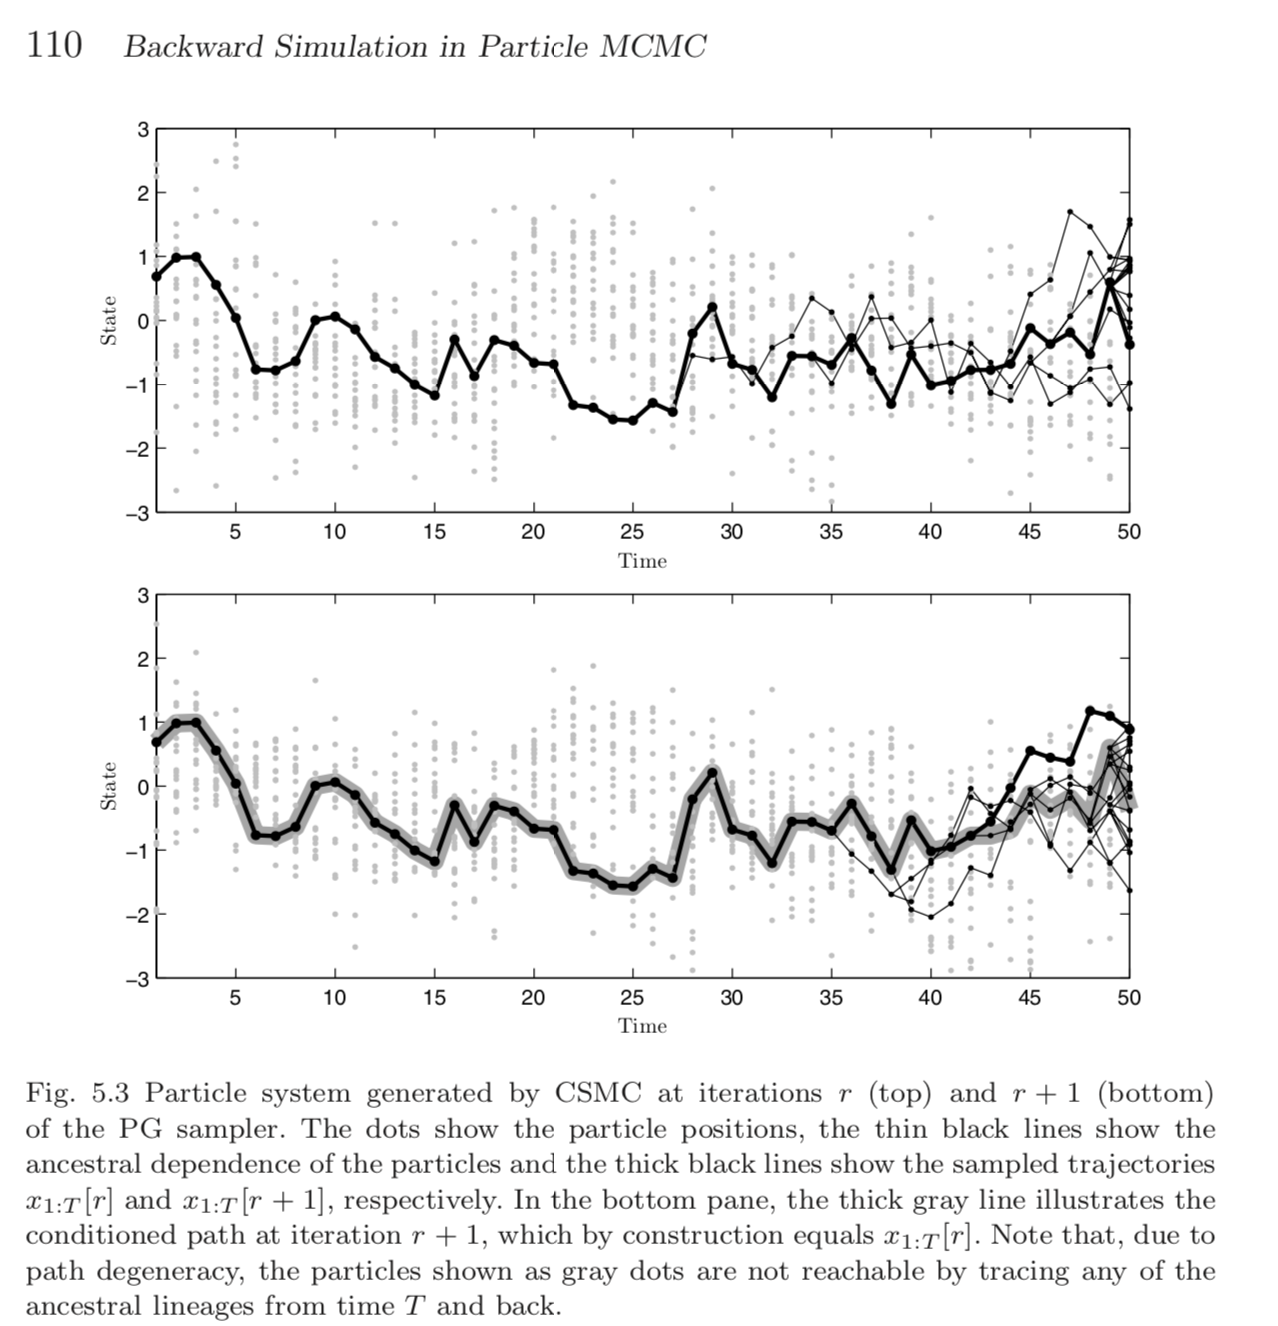
\includegraphics[width=0.8\textwidth]{plots/lindsten_figure.png}
\caption{PLACEHOLDER. Copied from \textcite{lindsten2013}.}
\label{fig:PG_ancdegen}
\end{figure}

To see why, take a look at Figure \ref{fig:PG_ancdegen}. In Figure \ref{fig:PG_ancdegen}a we have just completed the $r^{th}$ Gibbs sweep, sampling $\theta[r]$ and $x_{0:T}[r]$. For the $(r+1)^{th}$ sweep, we take as immortal trajectory $x_{0:T}^* = x_{0:T}[r]$, and run conditional SMC. Due to ancestral degeneracy, many of the resulting trajectories coalesce, and since the immortal trajectory must survive across the whole time window, they tend to coalesce onto the immortal trajectory (Figure \ref{fig:PG_ancdegen}b). Now we obtain the next sample $x_{0:T}[r+1]$ by sampling a trajectory among the $N$ we have just simulated. Whichever one we choose, it has a high amount of overlap with the immortal trajectory, i.e.\ the previous sample $x_{0:T}[r]$. This behaviour tends to repeat at every iteration, meaning the early $X$ coordinates are getting `stuck' (rarely being updated). This is clearly a problem for the mixing of the Markov chain.
\seb{Another way to explain this is that the variables defining the immortal trajectory (indices and states) are never refreshed during the Gibbs sweep - this is the explanation given in Lindsten Ch5.}
It renders the particle Gibbs algorithm impractical for any such model where the time horizon $T$ is too large: either we must run the Markov chain for longer, or increase the number of particles $N$ in the conditional SMC step, neither of which is feasible on a limited computational budget. 


\subsubsection{The solution: ancestor sampling}

An effective solution (where it is possible to implement it) was proposed by Nick Whiteley and is known as ancestor sampling.
It consists of a simple modification to the resampling step within the conditional SMC algorithm. 
In the basic CSMC algorithm, at each time step the particles are resampled by multinomial resampling according to their weights. That is, at each time $t$, each non-immortal offspring is assigned a parent as so:
\begin{equation*}
\Prob[a_t^{(j)} = i] \propto w_t^{(i)} ,
\end{equation*}
while the immortal offspring is deterministically assigned to the immortal parent.

\begin{figure}
\centering
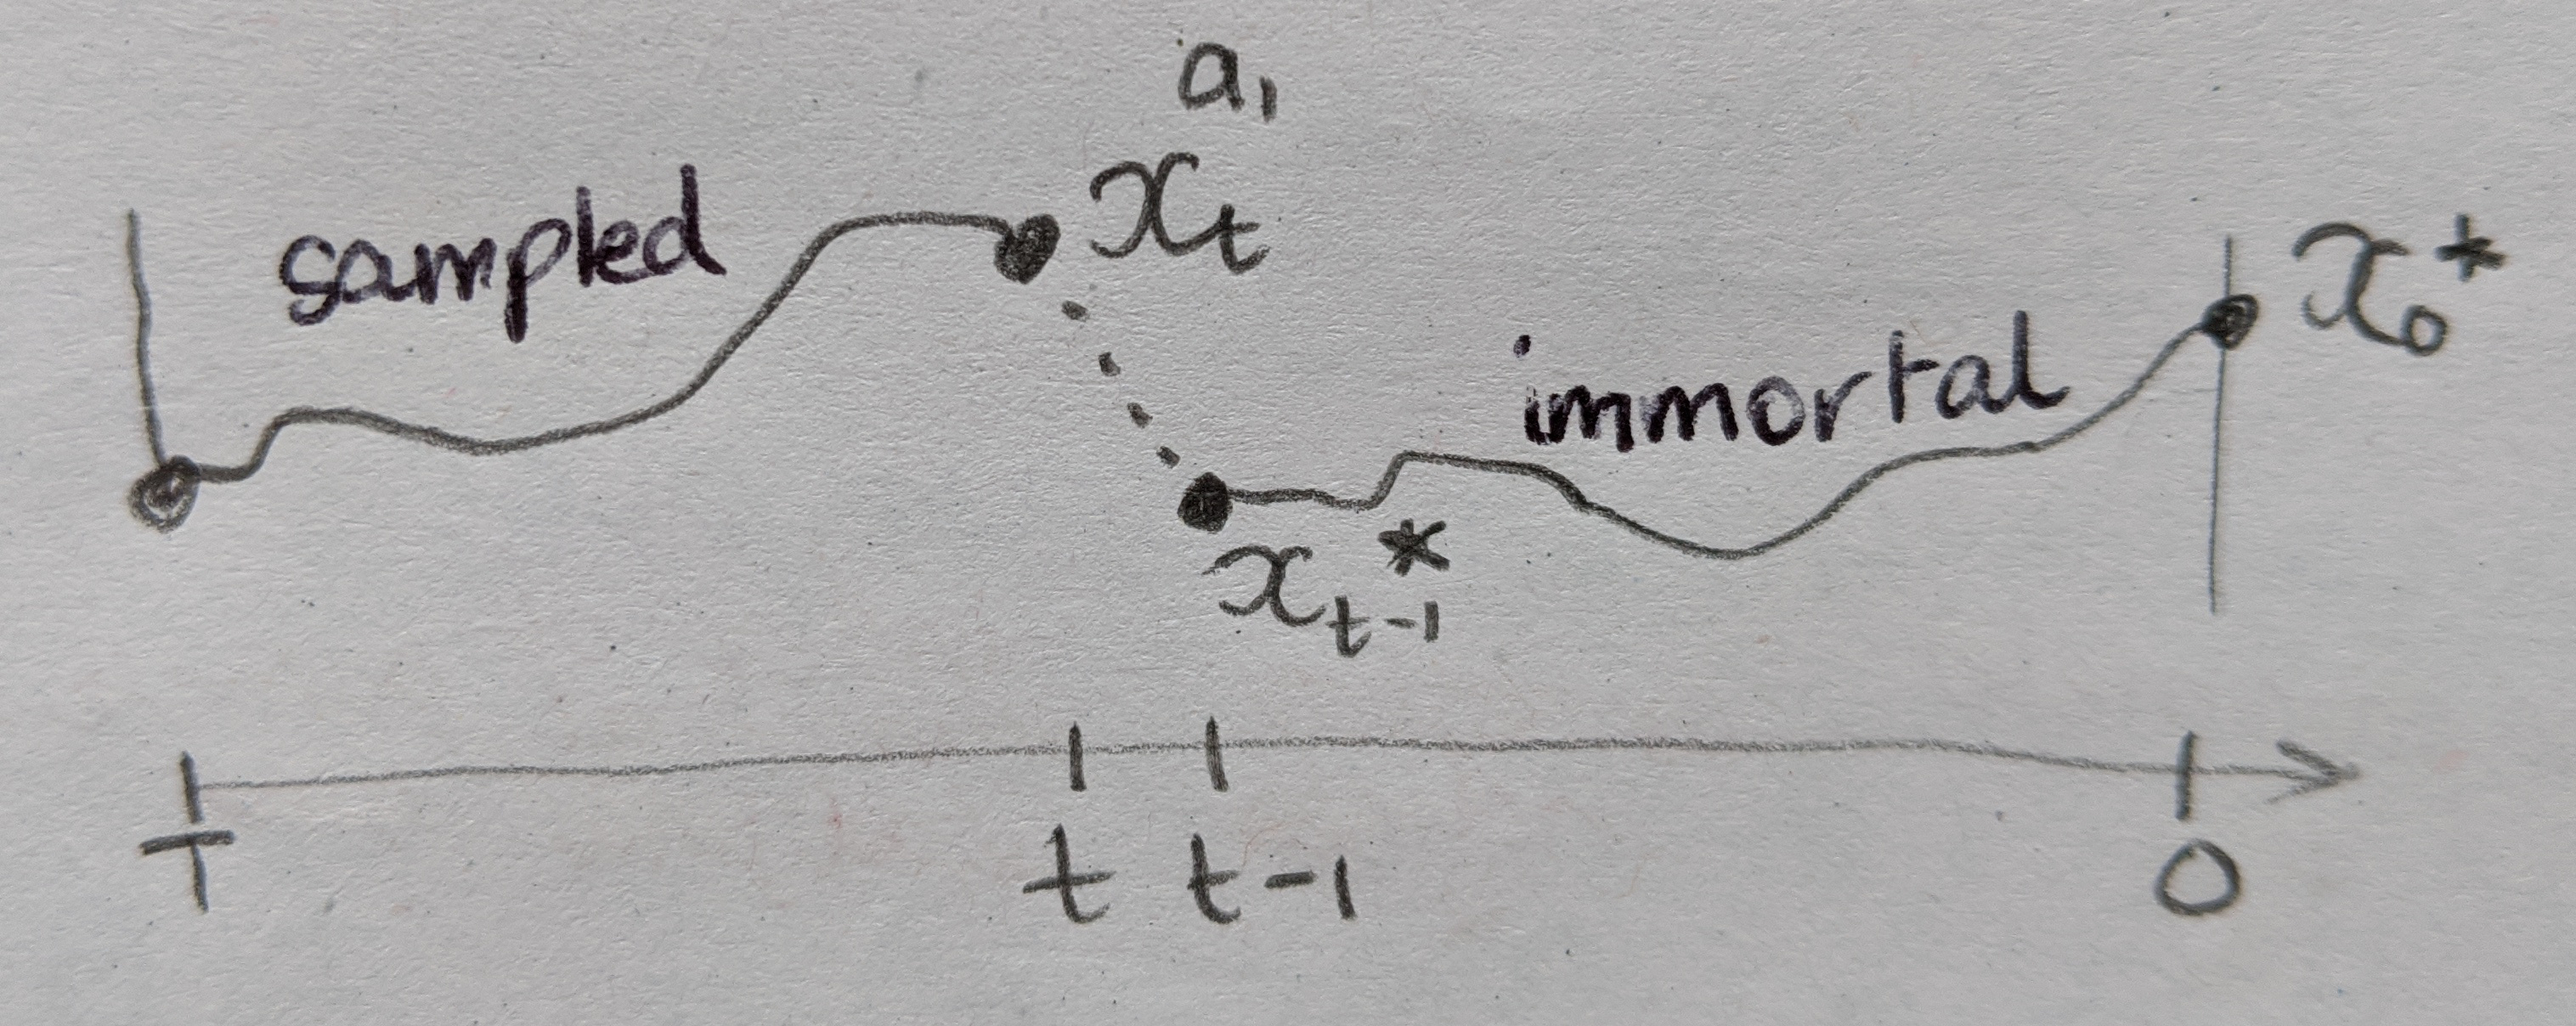
\includegraphics[width=0.8\textwidth]{plots/immresample.jpg}
\caption{PLACEHOLDER. Interpretation of a resampling weight for the immortal offspring.}
\label{fig:resample_immortal}
\end{figure}

In ancestor sampling we do the same thing, except that the immortal particle is also resampled, rather than being deterministically assigned:
\begin{equation*}
\Prob[a_t^{(j)} = i] \propto
\begin{cases}
w_t^{(i)} &\text{non-immortal particles}\\
w_t^{(i)} \frac{\gamma_T^\theta((x_{0:t-1}^{(i)}, x_{t:T}^*))}{\gamma_{t-1}^\theta(x_{0:t-1}^{(i)})} &\text{immortal particle} .
\end{cases}
\end{equation*}
The ratio of $\gamma$s can be interpreted as the conditional probability of the trajectory continuing with $x_{t:T}^*$ given is starts with $x_{0:t-1}^{(i)}$ (see Figure \ref{fig:resample_immortal}).
Using the structure of the hidden Markov model defined earlier, we can rewrite the ratio
\begin{equation*}
\frac{\gamma_T^\theta((x_{0:t-1}^{(i)}, x_{t:T}^*))}{\gamma_{t-1}^\theta(x_{0:t-1}^{(i)})}
\propto f_\theta(x_t^* \mid x_{t-1}^{(i)}) g_\theta(y_t \mid x_t^*) \prod_{s=t}^T f_\theta(x_r^* \mid x_{r-1}^*) g_\theta(y_r \mid x_r^*)
\propto f_\theta(x_t^* \mid x_{t-1}^{(i)}) .
\end{equation*}
\seb{Should the first propto actually be equality?}
So it looks like it should also be pretty easy to implement ancestor sampling for our model. \seb{Write down the pseudocode to prove it?}
The only catch is that we need to be able to evaluate $f_\theta$ pointwise, whereas in the basic algorithm we only need to draw samples from $f_\theta$. This will rule out ancestor sampling in some applications.


\subsubsection{Why ancestor sampling works}

Ancestor sampling is backward sampling, but only for the immortal trajectory. (It isn't possible to do backward sampling during the forward sweep for any except the immortal trajectory - see that we can't evaluate the required $\gamma$s without knowing the future states, which are known only for the immortal trajectory.)
We know that backward sampling (on all trajectories, in a separate backward sweep) eradicates ancestral degeneracy. But we've only backward-sampled one trajectory, leaving the other $N-1$ trajectories to do their coalescing thing.

The important point is that ancestor sampling does not prevent ancestral degeneracy (it mitigates it a tiny bit like $1/N$). Ancestral degeneracy is pretty much as severe as ever; the difference is that the trajectories no longer coalesce preferentially onto the immortal trajectory. There is no longer an immortal trajectory to coalesce onto. An illustration of this can be seen in Figure \ref{fig:whyASworks}.

\begin{figure}
\centering
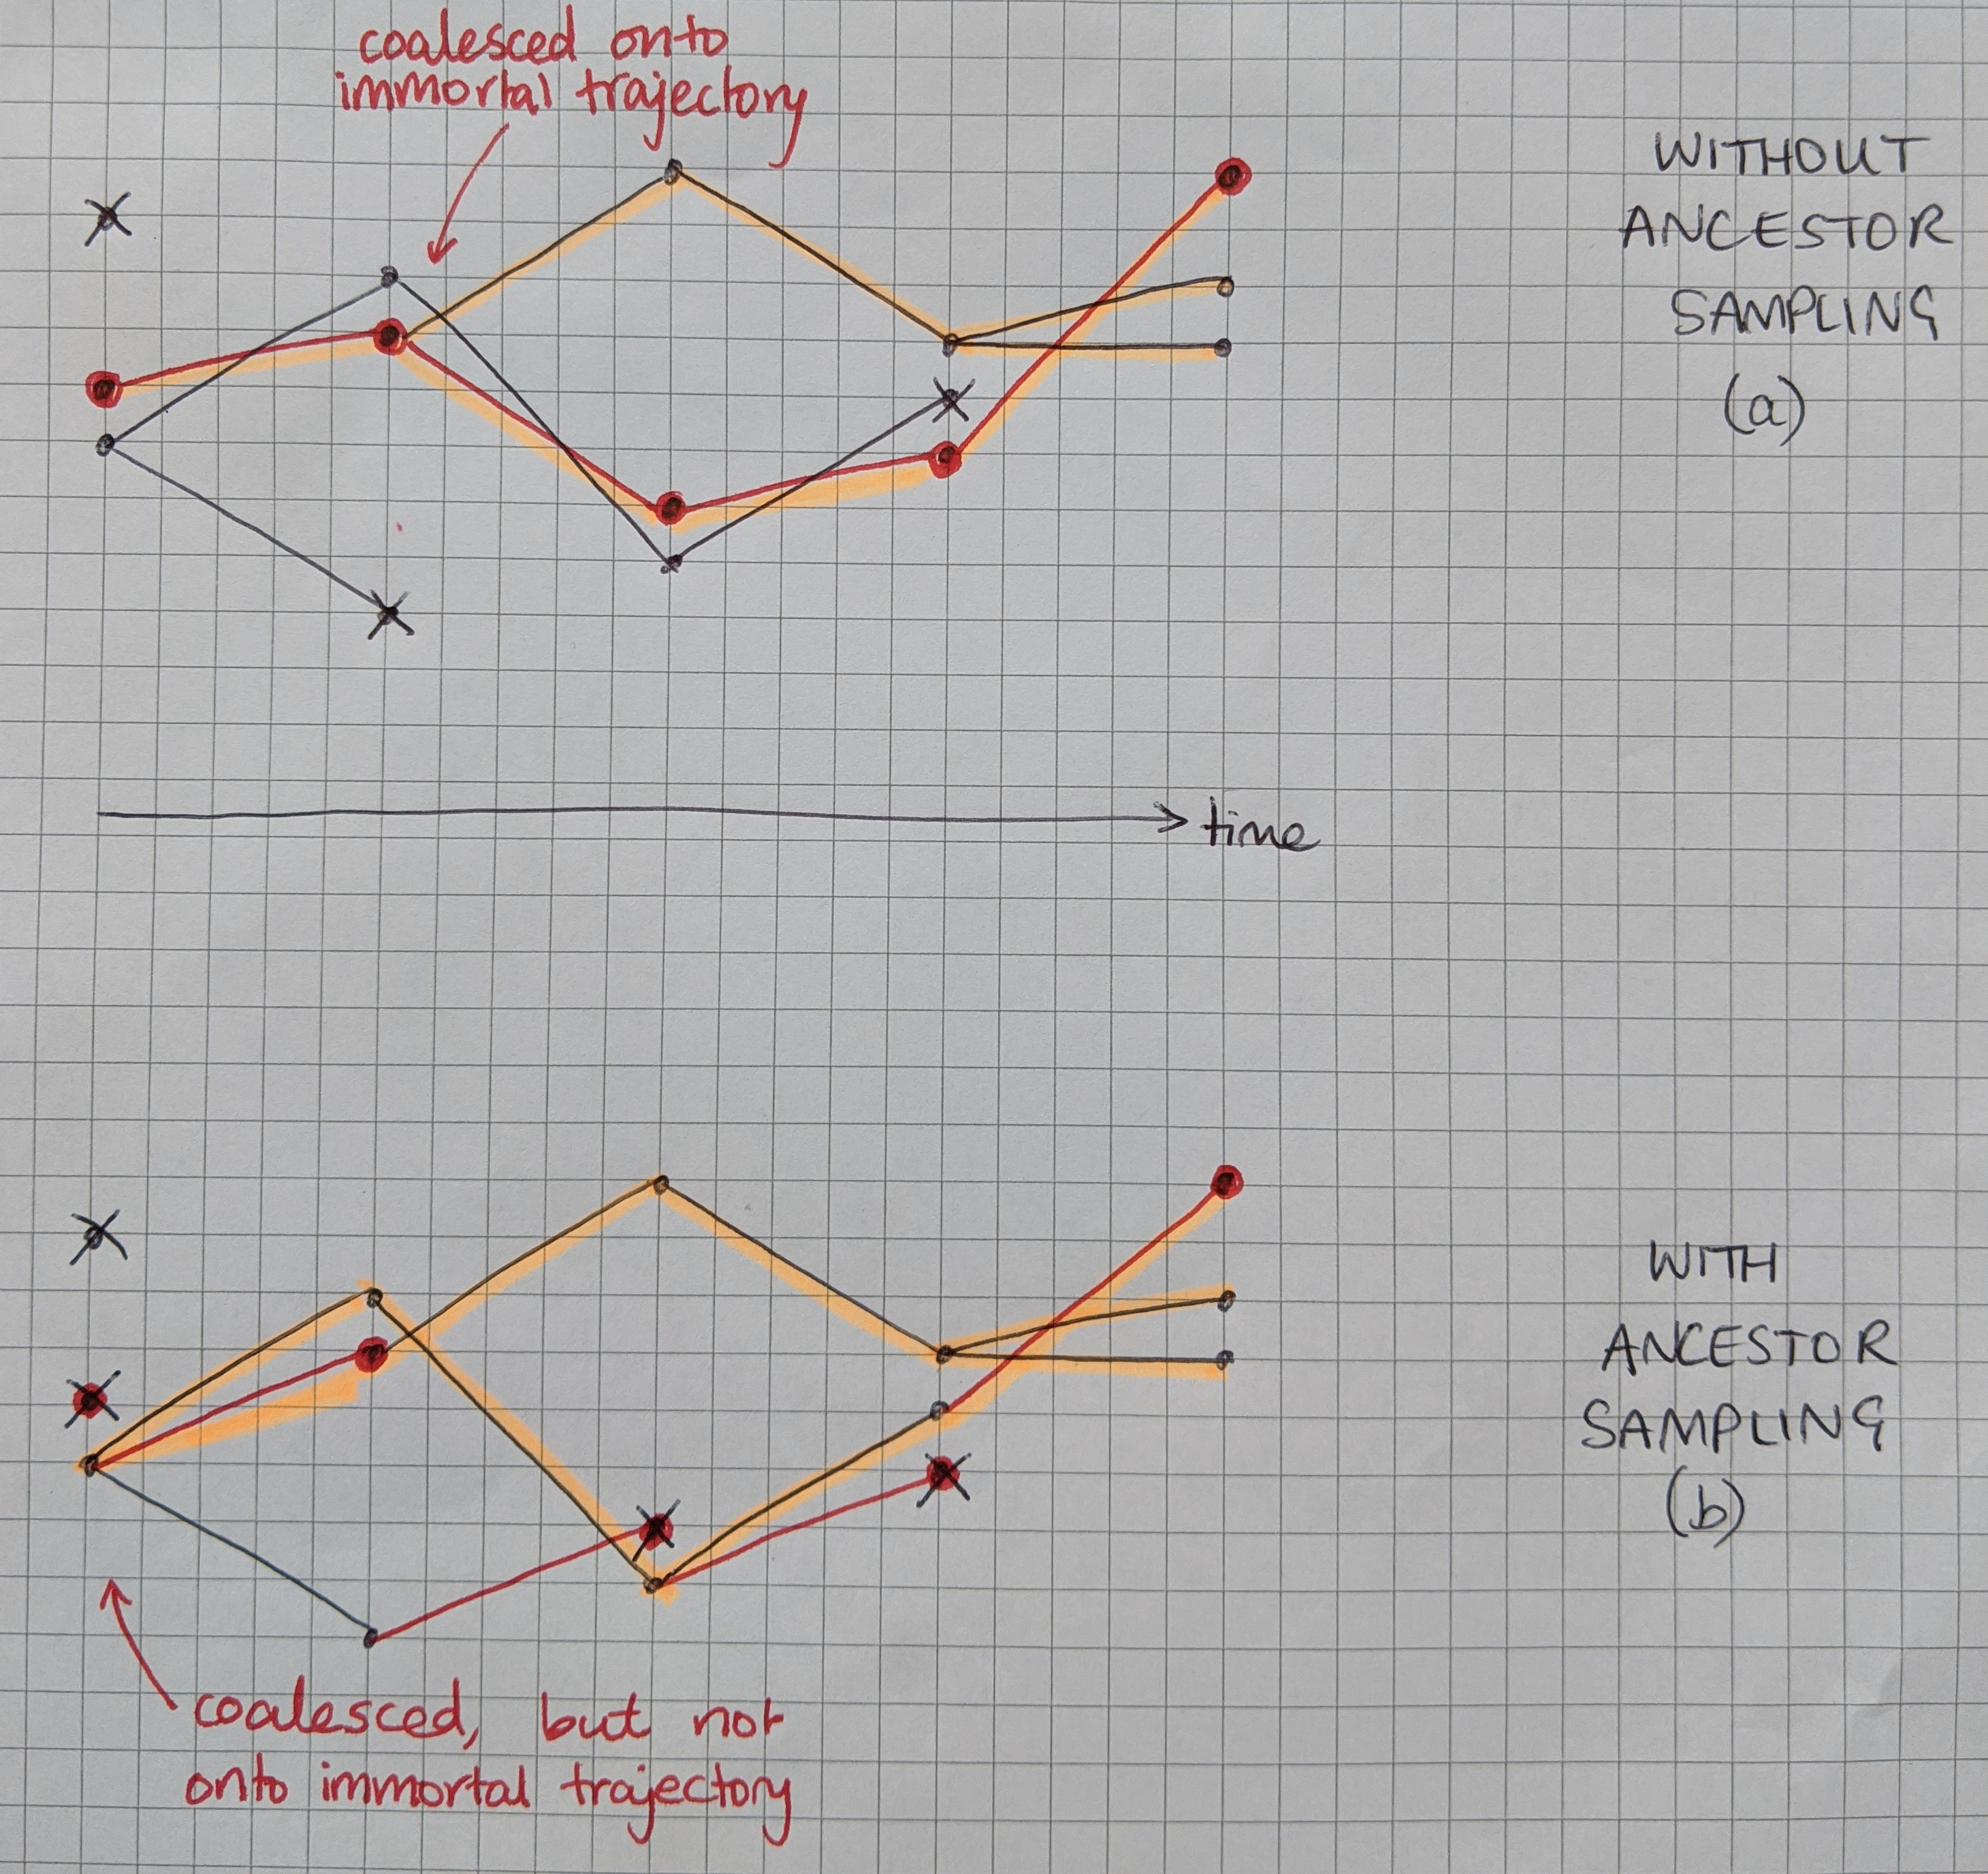
\includegraphics[width=0.8\textwidth]{plots/ancsampworks.jpg}
\caption{PLACEHOLDER. Illustration of how ancestor sampling prevents coalescence onto the immortal trajectory.}
\label{fig:whyASworks}
\end{figure}

Remember, the problem with ancestral degeneracy in particle Gibbs was that it induced strong autocorrelation among consecutive samples of $X_{0:T}$. It isn't a problem that the trajectories coalesce, as long as the thing they coalesce to is able to move, readily exploring the state space. This is achieved with ancestor sampling.

\seb{Why is ancestor sampling even a valid thing to do (i.e. still targetting the right thing)? Extended state space argument?(I think there is one in Lindsten Ch5). No need to go into it here unless there is a simple intuitive explanation to put the reader's mind at rest.}
